%! Author = crist
%! Date = 25/10/2026

\spacing{1.3}
%----------------------------------------------------------------------------------------
%	UNIDAD 7: LOS MOVIMIENTOS RECTILÍNEOS (4.º ESO)
%   Figuras: images/UD7/*.pdf (fuente HTML en images/UD7/html, SVG en images/UD7/svg)
%   Las gráficas de los ejercicios se dibujan con pgfplots (estilo «grafica»).
%----------------------------------------------------------------------------------------

%------------------------------------------------
% Estilo de las gráficas de la unidad
%------------------------------------------------
\pgfplotsset{grafica/.style={
    width=7.5cm, height=5.2cm, axis lines=left, grid=both,
    grid style={line width=.1pt, draw=gray!20}, major grid style={line width=.3pt, draw=gray!40},
    label style={font=\small}, tick label style={font=\footnotesize},
    /pgf/number format/use comma,
    every axis plot/.append style={line width=1.4pt, color=red!75!black, mark=*, mark size=1.6pt}}}

% Mapa conceptual del tema (fuente en images/mapas_conceptuales/html/temas.js)
\begin{figure}[H]
    \centering
    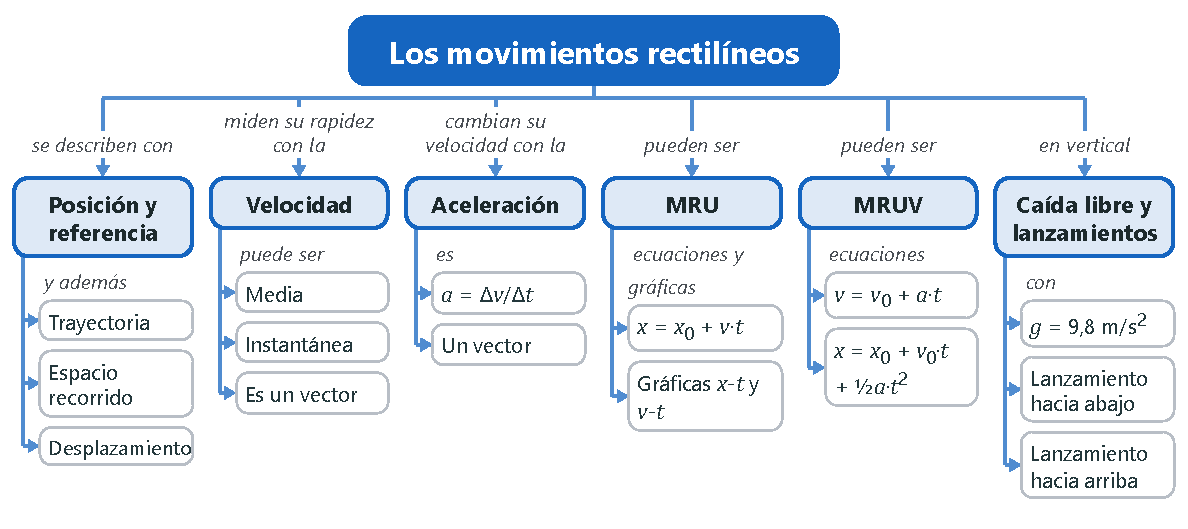
\includegraphics[width=\textwidth]{images/mapas_conceptuales/mapa_UD7}
\end{figure}

%========================================================================================
%\section*{Para empezar: batir un récord}
%\addcontentsline{toc}{section}{Para empezar: batir un récord}
%========================================================================================
%
%La experiencia dice que todos los récords acaban cayendo tarde o temprano. La superación de los deportistas y la mejora de los materiales, como las zapatillas, lo hacen posible. El 22 de julio de 2022, la estadounidense \textbf{Sydney McLaughlin} batió el récord mundial de los \qty{400}{\m} vallas con \qty{50.68}{\s}: superó diez vallas, las dos primeras con la pierna izquierda y las seis siguientes con la derecha, y mantuvo hasta el final un ritmo regular de 15 zancadas entre valla y valla. (En los Juegos de París 2024 lo rebajó todavía más, hasta \qty{50.37}{\s}.)
%
%Otro récord legendario es el de \textbf{Usain Bolt}, que en agosto de 2009 corrió los \qty{100}{\m} lisos en \qty{9.58}{\s}, una marca que nadie ha superado aún.
%
%Las hazañas de las deportistas tienen relación con el \textbf{ODS 5} (\emph{Igualdad de género}), cuya meta 5.5 busca asegurar la participación plena de las mujeres y la igualdad de oportunidades de liderazgo en todos los ámbitos. Los medios de comunicación deportivos pueden contribuir mucho a hacerlo visible.
%
%\begin{exercise}
%    ¿Qué velocidad media llevó Sydney McLaughlin en su carrera de 2022? ¿Y Usain Bolt en su récord de los \qty{100}{\m}? Expresa los resultados en \unit{\m\per\s} y en \unit{\km\per\hour}.
%    \begin{solu}
%        \textcolor{blue}{\(v_m = \dfrac{\text{espacio recorrido}}{\text{tiempo}}\); para pasar a km/h se multiplica por \num{3.6}.}
%        McLaughlin: \(v_m = \dfrac{400}{\num{50.68}} = \textcolor{red}{\qty{7.89}{\m\per\s}} = \qty{28.4}{\km\per\hour}\).
%        Bolt: \(v_m = \dfrac{100}{\num{9.58}} = \textcolor{red}{\qty{10.44}{\m\per\s}} = \qty{37.6}{\km\per\hour}\).
%    \end{solu}
%\end{exercise}
%
%\begin{exercise}
%    ¿Crees que McLaughlin mantuvo la misma velocidad durante toda la carrera? Además de la forma física, ¿pueden influir el calzado o el equipamiento en un récord?
%    \begin{solu}
%        \textcolor{red}{No}: mantuvo una cadencia regular de zancadas entre las vallas, pero la velocidad no fue constante (en la salida acelera desde el reposo y al saltar cada valla la velocidad cambia). Sí influyen el diseño y los materiales del calzado y del equipamiento (más ligeros, con mejor amortiguación y retorno de energía).
%    \end{solu}
%\end{exercise}
%
%\begin{exercise}
%    Algunos factores que influyen en una carrera son el tiempo de reacción en la salida, la capacidad de aceleración, la velocidad máxima y la capacidad de mantenerla. Debatid en clase la importancia de cada uno. ¿Qué pasos incluiríais en una agenda para alcanzar la meta 5.5 del ODS 5?
%    \begin{solu}
%        Respuesta libre.
%    \end{solu}
%\end{exercise}

%========================================================================================
\section{Posición, trayectoria y desplazamiento}
%========================================================================================

Si esperas el autobús en la parada, ves fácilmente si un coche está parado o se mueve. Pero desde dentro del autobús en marcha, ¿está en movimiento el asiento de al lado? Depende de \emph{respecto a qué} lo observes.

\subsection{Posición y sistema de referencia}

Un cuerpo en movimiento se llama \textbf{móvil}. Para describir su posición en cada instante necesitamos un \textbf{sistema de referencia}: en Física, unos ejes de coordenadas con un origen O. En el plano, la posición de un punto P queda determinada por sus coordenadas \((x, y)\).

\begin{definition}[Movimiento]
    Un cuerpo está en \textbf{movimiento} cuando su posición respecto a un sistema de referencia cambia con el tiempo. Si no cambia, está en \textbf{reposo}. El movimiento es, por tanto, \textbf{relativo}: depende del sistema de referencia elegido.
\end{definition}

\paragraph{El vector de posición.} La posición del punto P también queda determinada por el \textbf{vector de posición} \(\vec{r}\), que tiene su origen en O y su extremo en P. Su módulo es la distancia de O a P:
\[ r = \sqrt{x^2 + y^2} \]

\begin{figure}[H]
    \centering
    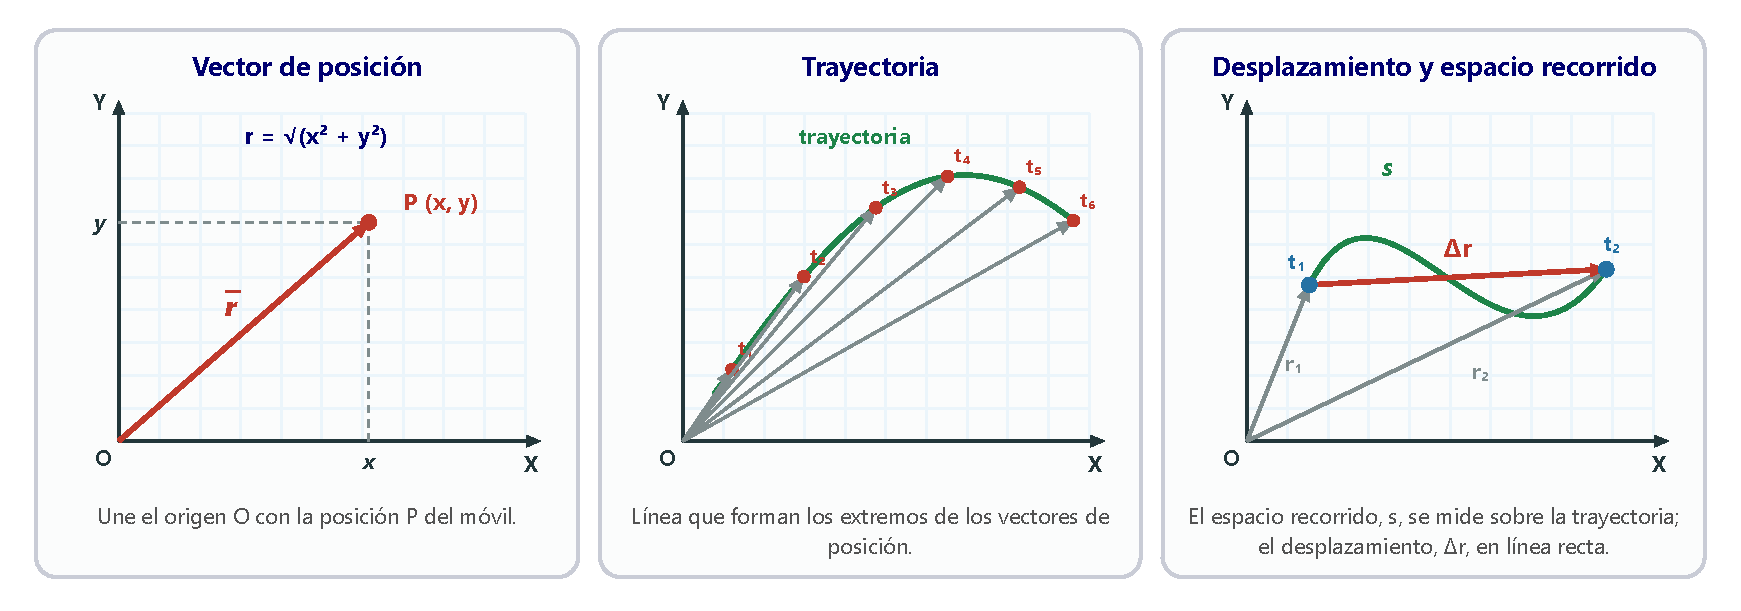
\includegraphics[width=\textwidth]{images/UD7/posicion_trayectoria}
    \caption{Vector de posición, trayectoria, desplazamiento y espacio recorrido.}
    \label{fig:posicion_trayectoria}
\end{figure}

\paragraph{Gráficas posición-tiempo.} En una gráfica posición-tiempo (\(x\)-\(t\)) se representa la posición del móvil en cada instante. En la del margen se lee que el móvil parte del origen, a los 2 s está en \(x = \qty{10}{\m}\), permanece en reposo hasta los 4 s, avanza hasta \(x = \qty{40}{\m}\) a los 6 s y vuelve al punto de partida en los 4 s siguientes.

\begin{center}
    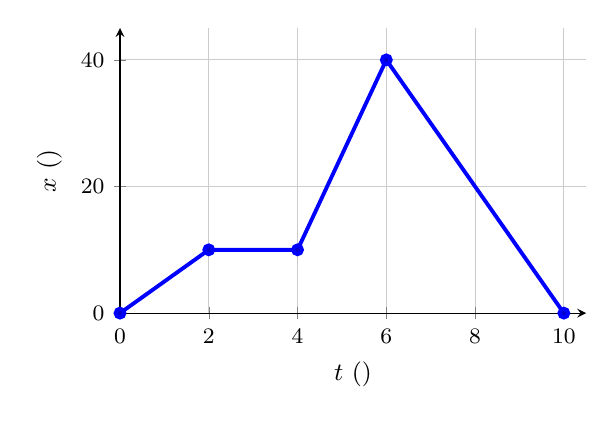
\begin{tikzpicture}
        \begin{axis}[grafica, xlabel={\(t\) (\unit{\s})}, ylabel={\(x\) (\unit{\m})}, xmin=0, xmax=10.5, ymin=0, ymax=45, xtick={0,2,...,10}]
            \addplot coordinates {(0,0) (2,10) (4,10) (6,40) (10,0)};
        \end{axis}
    \end{tikzpicture}
\end{center}

\subsection{La trayectoria y el espacio recorrido}

\begin{definition}[Trayectoria y espacio recorrido]
    La \textbf{trayectoria} es la línea imaginaria que describe un móvil al desplazarse, formada por todas las posiciones por las que pasa. La longitud medida sobre la trayectoria es el \textbf{espacio recorrido}, \(s\), una magnitud \textbf{escalar} que se mide en metros.
\end{definition}

Según su trayectoria, los movimientos se clasifican en \textbf{rectilíneos}, si la trayectoria es una recta, y \textbf{curvilíneos}, si no lo es. Entre estos últimos están los \textbf{circulares}, los \textbf{elípticos} y los \textbf{parabólicos} (figura~\ref{fig:tipos_trayectoria}).

\begin{figure}[H]
    \centering
    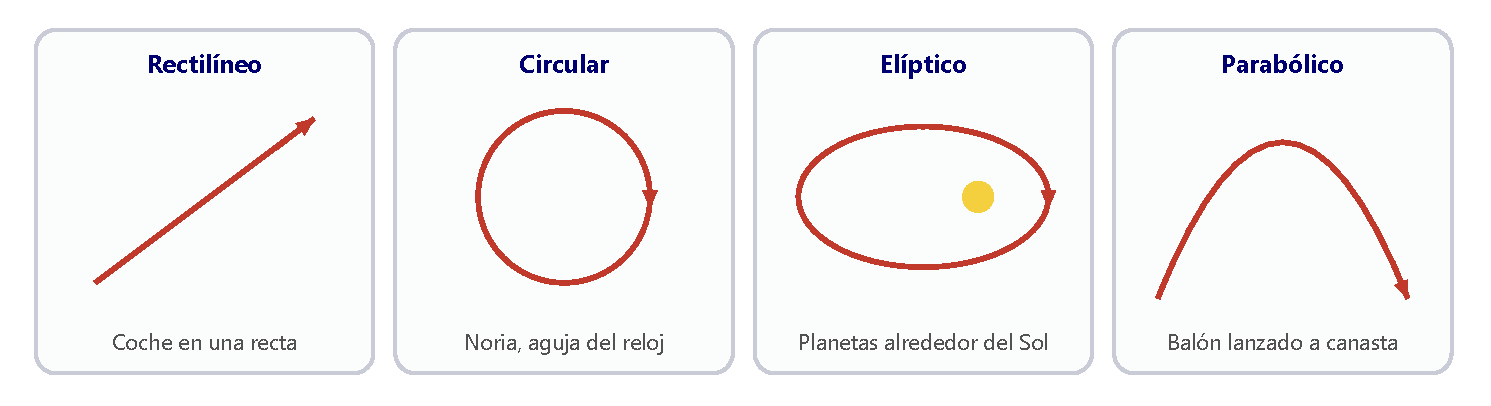
\includegraphics[width=0.95\textwidth]{images/UD7/tipos_trayectoria}
    \caption{Clasificación de los movimientos según su trayectoria.}
    \label{fig:tipos_trayectoria}
\end{figure}

\subsection{El desplazamiento}

Tres corredoras salen a la vez de la línea de salida. A los 5 segundos se han desplazado \qty{45}{\m}, \qty{35}{\m} y \qty{40}{\m}, respectivamente (figura~\ref{fig:corredoras}).

\begin{figure}[H]
    \centering
    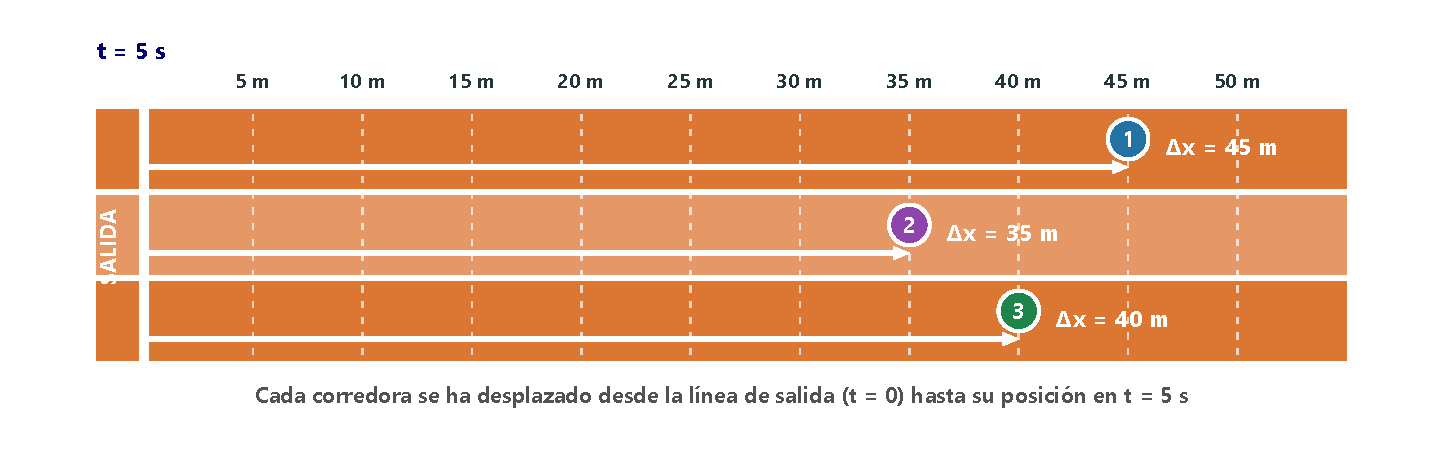
\includegraphics[width=\textwidth]{images/UD7/corredoras}
    \caption{Desplazamiento de tres corredoras al cabo de 5 segundos.}
    \label{fig:corredoras}
\end{figure}

\begin{definition}[Desplazamiento]
    El \textbf{desplazamiento} es la diferencia entre las posiciones de un móvil en dos instantes: \(\Delta x = x_2 - x_1\). Es un \textbf{vector} (\(\Delta\vec{r} = \vec{r}_2 - \vec{r}_1\)) que va de la posición inicial a la final y se mide en metros.
\end{definition}

El desplazamiento y el espacio recorrido no son lo mismo:
\begin{itemize}
    \item En un movimiento \textbf{curvilíneo}, el espacio recorrido sobre la trayectoria es mayor que el módulo del desplazamiento.
    \item En un movimiento \textbf{rectilíneo sin cambio de sentido}, ambos coinciden.
    \item Si un móvil \textbf{vuelve al punto de partida} (por ejemplo, un caballito de un tiovivo que da una vuelta completa), su desplazamiento es nulo, aunque el espacio recorrido no lo sea.
\end{itemize}

\begin{exercise}
    Dibuja un sistema de coordenadas y sitúa en él los puntos A(4, 1), B(\(-2\), 3), C(\(-3\), \(-2\)) y D(2, \(-4\)) (en metros). Dibuja sus vectores de posición y calcula sus módulos.
    \begin{solu}
        \[ r_A = \sqrt{4^2 + 1^2} = \textcolor{red}{\qty{4.12}{\m}} \qquad r_B = \sqrt{(-2)^2 + 3^2} = \textcolor{red}{\qty{3.61}{\m}} \]
        \[ r_C = \sqrt{(-3)^2 + (-2)^2} = \textcolor{red}{\qty{3.61}{\m}} \qquad r_D = \sqrt{2^2 + (-4)^2} = \textcolor{red}{\qty{4.47}{\m}} \]
    \end{solu}
\end{exercise}

\begin{exercise}
    Dibuja el vector de posición del punto (6, 8) m. ¿Cuál es su módulo?
    \begin{solu}
        \(r = \sqrt{6^2 + 8^2} = \sqrt{100} = \textcolor{red}{\qty{10}{\m}}\).
    \end{solu}
\end{exercise}

\begin{exercise}
    Representa en una gráfica posición-tiempo los datos de esta tabla y describe el movimiento:
    \begin{center}
        % --- tabla antigua ---
        % \begin{tblr}{colspec={lccccccccc}, hlines, vlines, column{1}={bg=ocre!85, fg=white, font=\bfseries}}
            % \(x\) (\unit{\m}) & 0 & 50 & 100 & 150 & 200 & 200 & 200 & 100 & 0 \\
            % \(t\) (\unit{\s}) & 0 & 5 & 10 & 15 & 20 & 25 & 30 & 35 & 40 \\
        % \end{tblr}
        % --- tabla nueva ---
        \begin{tabular}{@{}lccccccccc@{}}
            \toprule
            \textbf{\(x\) (\unit{\m})} & 0 & 50 & 100 & 150 & 200 & 200 & 200 & 100 & 0 \\[3pt]
            \textbf{\(t\) (\unit{\s})} & 0 & 5 & 10 & 15 & 20 & 25 & 30 & 35 & 40 \\
            \bottomrule
        \end{tabular}
    \end{center}
    \begin{solu}
        \begin{center}
            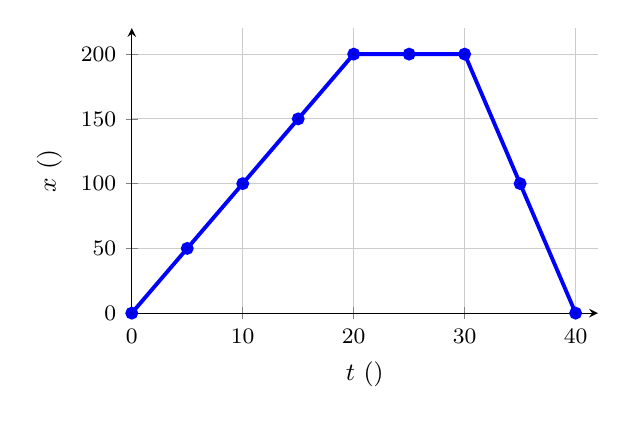
\begin{tikzpicture}
                \begin{axis}[grafica, xlabel={\(t\) (\unit{\s})}, ylabel={\(x\) (\unit{\m})}, xmin=0, xmax=42, ymin=0, ymax=220]
                    \addplot coordinates {(0,0) (5,50) (10,100) (15,150) (20,200) (25,200) (30,200) (35,100) (40,0)};
                \end{axis}
            \end{tikzpicture}
        \end{center}
        De 0 a 20 s el móvil se aleja del origen avanzando \qty{50}{\m} cada 5 s (\qty{10}{\m\per\s}); de 20 a 30 s está en \textcolor{red}{reposo} a \qty{200}{\m}; de 30 a 40 s \textcolor{red}{vuelve} al origen más deprisa (\qty{200}{\m} en \qty{10}{\s}, \qty{20}{\m\per\s}).
    \end{solu}
\end{exercise}

\begin{exercise}
    ¿Qué diferencia hay entre trayectoria y espacio recorrido? ¿Y entre espacio recorrido y desplazamiento?
    \begin{solu}
        La \textcolor{red}{trayectoria} es la línea que describe el móvil; el \textcolor{red}{espacio recorrido} es la longitud medida sobre esa línea. El \textcolor{red}{desplazamiento} es un vector que une la posición inicial con la final en línea recta, independientemente del camino seguido.
    \end{solu}
\end{exercise}

\begin{exercise}
    Describe la trayectoria de estos movimientos:
    \begin{enumerate}[label=\alph*)]
        \item una pelota que se deja caer;
        \item una piedra que gira atada a una cuerda;
        \item la punta del minutero de un reloj;
        \item una bolita de papel lanzada con un tirachinas;
        \item una atleta en una carrera de \qty{100}{\m} lisos;
        \item una atleta en una carrera de \qty{400}{\m}.
    \end{enumerate}
    \begin{solu}
        a) \textcolor{red}{Rectilínea} (vertical). b) y c) \textcolor{red}{Circular}. d) \textcolor{red}{Parabólica}. e) \textcolor{red}{Rectilínea}. f) \textcolor{red}{Curvilínea}: dos rectas y dos semicircunferencias.
    \end{solu}
\end{exercise}

\begin{exercise}
    Indica si son verdaderas o falsas y corrige las falsas:
    \begin{enumerate}[label=\alph*)]
        \item En una gráfica posición-tiempo se dibuja la trayectoria del móvil.
        \item Todos los movimientos curvilíneos son circulares.
        \item El desplazamiento es la trayectoria que sigue el móvil entre dos instantes.
    \end{enumerate}
    \begin{solu}
        a) \textcolor{red}{Falsa}: se representa cómo cambia la posición con el tiempo, no la forma del camino. b) \textcolor{red}{Falsa}: también hay movimientos elípticos, parabólicos\ldots{} c) \textcolor{red}{Falsa}: es la diferencia entre las posiciones final e inicial (un vector), no el camino seguido.
    \end{solu}
\end{exercise}

\begin{exercise}
    Pon dos ejemplos de movimientos rectilíneos, dos de circulares y uno de elíptico.
    \begin{solu}
        Respuesta libre. Rectilíneos: un tren en una vía recta, un objeto que cae. Circulares: una noria, un punto de un ventilador. Elíptico: la Tierra alrededor del Sol, un cometa.
    \end{solu}
\end{exercise}

\begin{exercise}
    Observa esta gráfica posición-tiempo:
    \begin{center}
        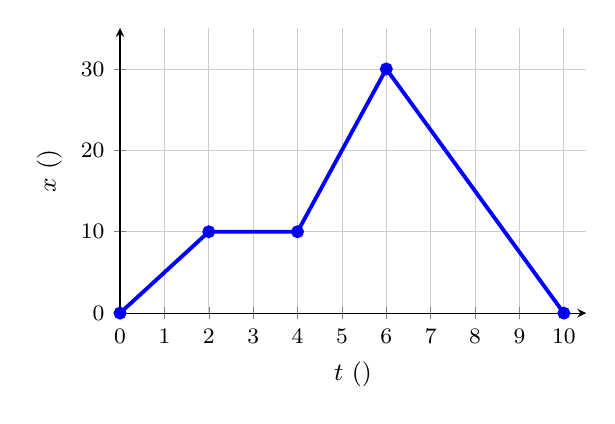
\begin{tikzpicture}
            \begin{axis}[grafica, xlabel={\(t\) (\unit{\s})}, ylabel={\(x\) (\unit{\m})}, xmin=0, xmax=10.5, ymin=0, ymax=35, xtick={0,1,...,10}]
                \addplot coordinates {(0,0) (2,10) (4,10) (6,30) (10,0)};
            \end{axis}
        \end{tikzpicture}
    \end{center}
    \begin{enumerate}[label=\alph*)]
        \item ¿Cuál ha sido el desplazamiento entre \(t = \qty{2}{\s}\) y \(t = \qty{6}{\s}\)?
        \item ¿Y el desplazamiento total?
        \item ¿Y en los cuatro últimos segundos?
        \item ¿Qué espacio total ha recorrido?
    \end{enumerate}
    \begin{solu}
        a) \(\Delta x = 30 - 10 = \textcolor{red}{\qty{20}{\m}}\). b) \(\Delta x = 0 - 0 = \textcolor{red}{0}\): vuelve al origen. c) \(\Delta x = 0 - 30 = \textcolor{red}{\qty{-30}{\m}}\) (el signo indica que se mueve hacia el origen). d) \(s = 30 + 30 = \textcolor{red}{\qty{60}{\m}}\).
    \end{solu}
\end{exercise}

\begin{exercise}
    Un móvil da una vuelta completa a una circunferencia de \qty{8}{\m} de radio. ¿Cuánto vale su desplazamiento? ¿Y el espacio recorrido?
    \begin{solu}
        El desplazamiento es \textcolor{red}{nulo}, porque vuelve al punto de partida. El espacio recorrido es la longitud de la circunferencia: \(s = 2\pi r = 2\pi \cdot 8 = \textcolor{red}{\qty{50.3}{\m}}\).
    \end{solu}
\end{exercise}

\begin{exercise}
    Calcula el espacio recorrido por un móvil que:
    \begin{enumerate}[label=\alph*)]
        \item se mueve en línea recta y sin cambiar de sentido desde \(x = \qty{-80}{\m}\) hasta \(x = \qty{520}{\m}\);
        \item da una vuelta completa a una pista circular de \qty{5}{\m} de radio.
    \end{enumerate}
    \begin{solu}
        a) \(s = 520 - (-80) = \textcolor{red}{\qty{600}{\m}}\). b) \(s = 2\pi \cdot 5 = \textcolor{red}{\qty{31.4}{\m}}\).
    \end{solu}
\end{exercise}

\begin{exercise}
    La punta del minutero de un reloj sale de las 12 y vuelve a pasar por las 12 una hora después.
    \begin{enumerate}[label=\alph*)]
        \item ¿Cómo es su trayectoria?
        \item ¿Cuál ha sido su desplazamiento?
    \end{enumerate}
    \begin{solu}
        a) \textcolor{red}{Circular}. b) \textcolor{red}{Nulo}, porque la posición final coincide con la inicial.
    \end{solu}
\end{exercise}

\begin{exercise}
    Un autobús está inicialmente a \qty{150}{\m} de una parada y se acerca a ella de forma uniforme; a los 20 s se detiene en la parada. Durante 20 s bajan los viajeros y después se aleja, de modo que 20 s más tarde está a \qty{150}{\m} de la parada. Representa la gráfica posición-tiempo tomando la parada como origen.
    \begin{solu}
        \begin{center}
            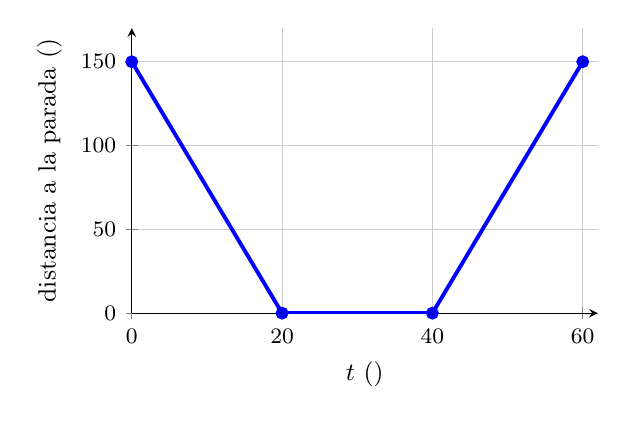
\begin{tikzpicture}
                \begin{axis}[grafica, xlabel={\(t\) (\unit{\s})}, ylabel={distancia a la parada (\unit{\m})}, xmin=0, xmax=62, ymin=0, ymax=170]
                    \addplot coordinates {(0,150) (20,0) (40,0) (60,150)};
                \end{axis}
            \end{tikzpicture}
        \end{center}
        \textcolor{blue}{Tres tramos:} se acerca (la distancia baja de 150 a 0), está parado (recta horizontal) y se aleja (la distancia sube de 0 a 150).
    \end{solu}
\end{exercise}

%========================================================================================
\section{¿Con qué rapidez cambia un móvil su posición? La velocidad}
%========================================================================================

En el ejemplo de las corredoras, la número 1 ha recorrido más distancia (\qty{45}{\m}) en el mismo tiempo (\qty{5}{\s}): es la más rápida. La magnitud que mide la rapidez con la que un cuerpo cambia de posición es la \textbf{velocidad}.

\subsection{La velocidad media}

\begin{definition}[Velocidad media]
    La \textbf{velocidad media} es el desplazamiento de un móvil dividido entre el tiempo empleado:
    \[ v_m = \frac{x - x_0}{t - t_0} = \frac{\Delta x}{\Delta t} \]
    Su unidad en el SI es el \textbf{metro por segundo} (\unit{\m\per\s}), aunque se usa mucho el \unit{\km\per\hour}.
\end{definition}

Si la trayectoria es rectilínea y el móvil no cambia de sentido, el desplazamiento coincide con el espacio recorrido y podemos escribir \(v_m = \dfrac{\Delta s}{\Delta t}\). Cuando no es así, al cociente entre el espacio recorrido y el tiempo se le llama \textbf{rapidez media}.

\begin{marker}
    \textbf{Conversión de unidades de velocidad.}
    \[ \qty{90}{\km\per\hour} = \frac{\qty{90}{\km}}{\qty{1}{\hour}} \cdot \frac{\qty{1000}{\m}}{\qty{1}{\km}} \cdot \frac{\qty{1}{\hour}}{\qty{3600}{\s}} = \qty{25}{\m\per\s} \qquad\qquad \qty{10}{\m\per\s} = \frac{\qty{10}{\m}}{\qty{1}{\s}} \cdot \frac{\qty{1}{\km}}{\qty{1000}{\m}} \cdot \frac{\qty{3600}{\s}}{\qty{1}{\hour}} = \qty{36}{\km\per\hour} \]
    Atajo: de \unit{\km\per\hour} a \unit{\m\per\s} se divide entre \num{3.6}; de \unit{\m\per\s} a \unit{\km\per\hour} se multiplica por \num{3.6}.
\end{marker}

\subsection{La velocidad instantánea}

Un ciclista recorre \qty{80}{\km} en \qty{2}{\hour}: su velocidad media es \qty{40}{\km\per\hour}. Pero seguro que en unos tramos fue más deprisa, en otros más despacio e incluso se detuvo alguna vez.

\begin{definition}[Velocidad instantánea]
    Es la velocidad de un móvil en un instante determinado o en un punto concreto de su trayectoria. Es la que marca el velocímetro de un coche.
\end{definition}

\begin{itemize}
    \item Si la velocidad instantánea es \textbf{constante} durante todo el movimiento, coincide con la media y el movimiento es \textbf{uniforme}.
    \item Si la velocidad instantánea \textbf{cambia}, el movimiento es \textbf{variado} (no uniforme).
\end{itemize}

\subsection{La velocidad es un vector}

Dos nadadoras salen a la vez del mismo punto a \qty{1.25}{\m\per\s}. ¿A qué distancia estarán a los 5 s? Si nadan en el mismo sentido, juntas; si nadan en sentidos contrarios, a \qty{12.5}{\m}. La velocidad, como el desplazamiento, es una magnitud \textbf{vectorial}: hay que indicar su módulo, su dirección y su sentido (figura~\ref{fig:velocidad_vector}).
\begin{itemize}
    \item El vector \textbf{velocidad media} tiene la dirección y el sentido del desplazamiento.
    \item El vector \textbf{velocidad instantánea} es \textbf{tangente} a la trayectoria en cada punto, apunta en el sentido del movimiento y se aplica en la posición del móvil. En un movimiento rectilíneo tiene la dirección de la propia trayectoria.
\end{itemize}

\begin{figure}[H]
    \centering
    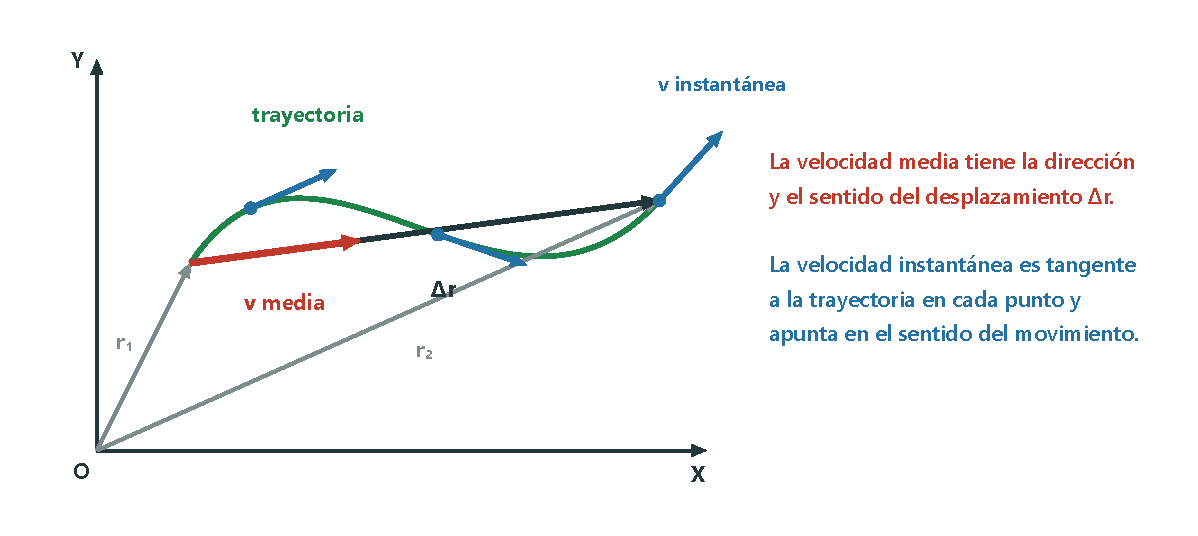
\includegraphics[width=0.85\textwidth]{images/UD7/velocidad_vector}
    \caption{Vectores velocidad media y velocidad instantánea.}
    \label{fig:velocidad_vector}
\end{figure}

\paragraph{Gráficas velocidad-tiempo.} En una gráfica \(v\)-\(t\) se lee la velocidad en cada instante. En la siguiente, el móvil parte del reposo y aumenta su velocidad hasta \qty{20}{\m\per\s} en 15 s (movimiento variado), la mantiene constante durante 15 s (movimiento uniforme) y frena hasta detenerse en 10 s (movimiento variado).

\begin{center}
    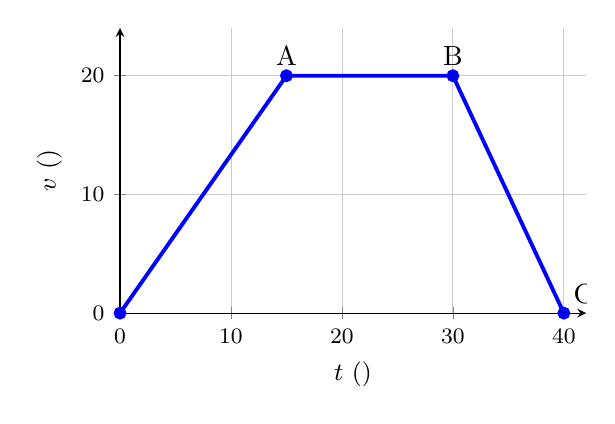
\begin{tikzpicture}
        \begin{axis}[grafica, xlabel={\(t\) (\unit{\s})}, ylabel={\(v\) (\unit{\m\per\s})}, xmin=0, xmax=42, ymin=0, ymax=24]
            \addplot coordinates {(0,0) (15,20) (30,20) (40,0)};
            \node[above] at (axis cs:15,20) {A}; \node[above] at (axis cs:30,20) {B}; \node[above right] at (axis cs:40,0) {C};
        \end{axis}
    \end{tikzpicture}
\end{center}

\begin{example}
    Una nadadora recorre una piscina de \qty{50}{\m} a \qty{1.25}{\m\per\s} constantes, descansa 30 s en el borde y vuelve al punto de salida a \qty{1}{\m\per\s}. Calcula el espacio recorrido, el desplazamiento, la rapidez media y la velocidad media en todo el recorrido.

    \textcolor{blue}{Tiempos:} \(t_1 = \dfrac{50}{\num{1.25}} = \qty{40}{\s}\); \(t_2 = \qty{30}{\s}\) (descanso); \(t_3 = \dfrac{50}{1} = \qty{50}{\s}\). Total: \qty{120}{\s}.

    \textcolor{blue}{Espacio recorrido:} \(s = 50 + 50 = \textcolor{red}{\qty{100}{\m}}\); \textcolor{blue}{rapidez media:} \(\dfrac{100}{120} = \textcolor{red}{\qty{0.83}{\m\per\s}}\).

    \textcolor{blue}{Desplazamiento:} \textcolor{red}{nulo}, porque vuelve al punto de partida; por tanto, la \textcolor{blue}{velocidad media} es \textcolor{red}{0}.
\end{example}

\begin{exercise}
    Ordena de mayor a menor estas velocidades:
    \begin{enumerate}[label=\alph*)]
        \item un caracol que recorre \qty{1}{\m} en 40 min;
        \item el sonido en el aire, \qty{340}{\m\per\s};
        \item una esquiadora que recorre \qty{6}{\km} en 20 min;
        \item la luz, \qty{3e8}{\m\per\s};
        \item un caballo que recorre \qty{15}{\km} en 30 min;
        \item un coche que recorre \qty{1.8}{\km} en 1 min.
    \end{enumerate}
    \begin{solu}
        \textcolor{blue}{Pasamos todas a m/s:} a) \(\frac{1}{2400} = \qty{4.2e-4}{\m\per\s}\); b) \qty{340}{\m\per\s}; c) \(\frac{6000}{1200} = \qty{5}{\m\per\s}\); d) \qty{3e8}{\m\per\s}; e) \(\frac{15000}{1800} = \qty{8.33}{\m\per\s}\); f) \(\frac{1800}{60} = \qty{30}{\m\per\s}\).
        \textcolor{red}{luz \(>\) sonido \(>\) coche \(>\) caballo \(>\) esquiadora \(>\) caracol}.
    \end{solu}
\end{exercise}

\begin{exercise}
    Explica la diferencia entre velocidad media y velocidad instantánea. ¿Cuándo coinciden?
    \begin{solu}
        La \textcolor{red}{media} es el desplazamiento total dividido entre el tiempo total; la \textcolor{red}{instantánea} es la velocidad en un instante concreto. Coinciden cuando el movimiento es \textcolor{red}{uniforme} (la velocidad no cambia).
    \end{solu}
\end{exercise}

\begin{exercise}
    En un campeonato, un nadador recorrió los \qty{50}{\m} libres en \qty{20.91}{\s} y los \qty{100}{\m} libres en \qty{46.40}{\s}. Calcula su velocidad media en cada prueba.
    \begin{solu}
        \(v_{50} = \frac{50}{\num{20.91}} = \textcolor{red}{\qty{2.39}{\m\per\s}}\); \quad \(v_{100} = \frac{100}{\num{46.40}} = \textcolor{red}{\qty{2.16}{\m\per\s}}\).
    \end{solu}
\end{exercise}

\begin{exercise}
    El atleta más rápido de tu clase recorre \qty{100}{\m} en \qty{15}{\s}. Calcula su velocidad media. ¿Qué distancia recorre de media cada segundo? ¿Crees que recorre realmente esa distancia en cada uno de los 15 segundos?
    \begin{solu}
        \(v_m = \frac{100}{15} = \textcolor{red}{\qty{6.67}{\m\per\s}}\): de media, \qty{6.67}{\m} cada segundo. \textcolor{red}{No}: parte del reposo, así que en los primeros segundos recorre menos y, cuando alcanza su velocidad máxima, más.
    \end{solu}
\end{exercise}

\begin{exercise}
    Halla la velocidad media de un vehículo que recorre \qty{3}{\km} en 2,5 minutos.
    \begin{solu}
        \(v_m = \frac{3000}{150} = \textcolor{red}{\qty{20}{\m\per\s}} = \qty{72}{\km\per\hour}\).
    \end{solu}
\end{exercise}

\begin{exercise}
    En 2023, el keniano Kelvin Kiptum corrió el maratón (\qty{42195}{\m}) en 2 h 0 min 35 s. ¿Cuál fue su velocidad media en \unit{\m\per\s} y en \unit{\km\per\hour}?
    \begin{solu}
        \(t = 2 \cdot 3600 + 35 = \qty{7235}{\s}\); \(v_m = \frac{42195}{7235} = \textcolor{red}{\qty{5.83}{\m\per\s}} = \textcolor{red}{\qty{21.0}{\km\per\hour}}\).
    \end{solu}
\end{exercise}

\begin{exercise}
    Halla la velocidad media de un caracol que recorre un metro en 25 minutos.
    \begin{solu}
        \(v_m = \frac{1}{1500} = \textcolor{red}{\qty{6.7e-4}{\m\per\s}}\) (unos \qty{2.4}{\m\per\hour}).
    \end{solu}
\end{exercise}

\begin{exercise}
    Luisa va en línea recta desde su casa hasta una tienda situada a \qty{300}{\m}, a \qty{1.5}{\m\per\s} constantes. Está 3 minutos en la tienda y vuelve a casa a \qty{2}{\m\per\s}.
    \begin{enumerate}[label=\alph*)]
        \item ¿Qué espacio ha recorrido?
        \item ¿Cuál ha sido su desplazamiento?
        \item ¿Cuál ha sido su rapidez media? ¿Y su velocidad media?
    \end{enumerate}
    \begin{solu}
        Tiempos: ida \(\frac{300}{\num{1.5}} = \qty{200}{\s}\); tienda \qty{180}{\s}; vuelta \(\frac{300}{2} = \qty{150}{\s}\). Total: \qty{530}{\s}.
        a) \(s = \textcolor{red}{\qty{600}{\m}}\). b) \textcolor{red}{Nulo}. c) Rapidez media: \(\frac{600}{530} = \textcolor{red}{\qty{1.13}{\m\per\s}}\); velocidad media: \textcolor{red}{0}, porque el desplazamiento es nulo.
    \end{solu}
\end{exercise}

\begin{exercise}
    Un atleta que prepara los \qty{1500}{\m} hace el recorrido en 3 min 45 s. ¿Cuál ha sido su velocidad media? ¿Crees que la ha mantenido todo el tiempo?
    \begin{solu}
        \(t = \qty{225}{\s}\); \(v_m = \frac{1500}{225} = \textcolor{red}{\qty{6.67}{\m\per\s}}\). \textcolor{red}{No}: en la salida tiene que acelerar y en el final suele cambiar de ritmo.
    \end{solu}
\end{exercise}

\begin{exercise}
    Un excursionista ve un relámpago y oye el trueno 6 s después. ¿A qué distancia está la tormenta? (Velocidad del sonido: \qty{340}{\m\per\s}; la luz llega prácticamente al instante.)
    \begin{solu}
        \(d = v \cdot t = 340 \cdot 6 = \textcolor{red}{\qty{2040}{\m}}\), unos \qty{2}{\km}.
    \end{solu}
\end{exercise}

%========================================================================================
\section{¿Cómo cambia la velocidad? La aceleración}
%========================================================================================

La velocidad de un móvil no suele ser constante: aumenta o disminuye con el tiempo.

\begin{definition}[Aceleración]
    La \textbf{aceleración} informa de cómo cambia la velocidad de un cuerpo con el tiempo. La \textbf{aceleración media} es la variación de la velocidad dividida entre el tiempo empleado:
    \[ a_m = \frac{v - v_0}{t - t_0} = \frac{\Delta v}{\Delta t} \]
    Su unidad en el SI es el \unit{\m\per\square\s} («metro por segundo al cuadrado»). La \textbf{aceleración instantánea} es la aceleración en un instante concreto.
\end{definition}

Si la aceleración instantánea es constante, coincide con la media y el movimiento es \textbf{uniformemente variado}: \textbf{acelerado} si la aceleración es positiva y \textbf{retardado} (o frenado) si es negativa. Una aceleración de \qty{2}{\m\per\square\s} significa que la velocidad aumenta \qty{2}{\m\per\s} cada segundo.

\begin{example}
    Un motorista que circula a \qty{72}{\km\per\hour} ve un obstáculo y detiene la moto en \qty{4}{\s}. ¿Cuál ha sido su aceleración? ¿Qué significa el signo?

    \textcolor{blue}{Pasamos a unidades del SI:} \(v_0 = \dfrac{72}{\num{3.6}} = \qty{20}{\m\per\s}\); \(v = 0\).
    \[ a = \frac{v - v_0}{t - t_0} = \frac{0 - 20}{4} = \textcolor{red}{\qty{-5}{\m\per\square\s}} \]
    El signo menos indica que la velocidad \textbf{disminuye}: es una aceleración de frenado.
\end{example}

\subsection{La aceleración es un vector}

Como la velocidad, la aceleración es una magnitud vectorial. En un movimiento rectilíneo:
\begin{itemize}
    \item Su \textbf{dirección} es la de la trayectoria (la misma que la del desplazamiento y la velocidad).
    \item Su \textbf{sentido} coincide con el de la velocidad si el movimiento es acelerado y es el contrario si es frenado (figura~\ref{fig:aceleracion_rampa}).
    \item Su \textbf{módulo} es \(a = \dfrac{v - v_0}{t - t_0}\).
\end{itemize}

\begin{figure}[H]
    \centering
    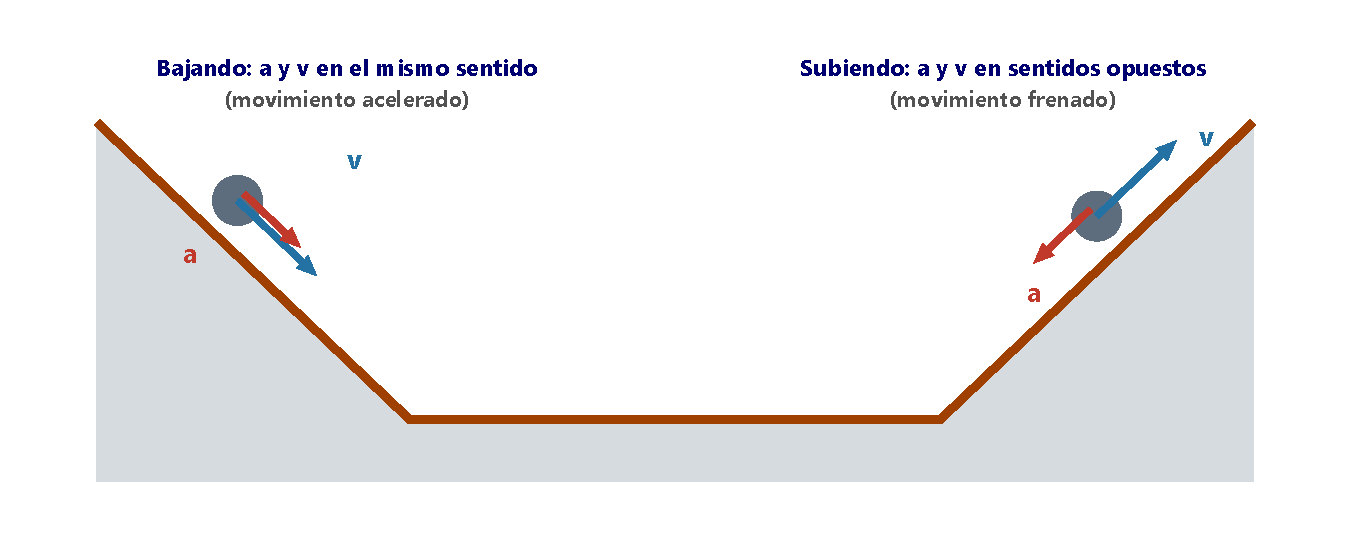
\includegraphics[width=0.9\textwidth]{images/UD7/aceleracion_rampa}
    \caption{Un monopatín en una rampa: al bajar se acelera y al subir se frena.}
    \label{fig:aceleracion_rampa}
\end{figure}

\begin{example}
    Calcula la aceleración en cada tramo de esta gráfica velocidad-tiempo:
    \begin{center}
        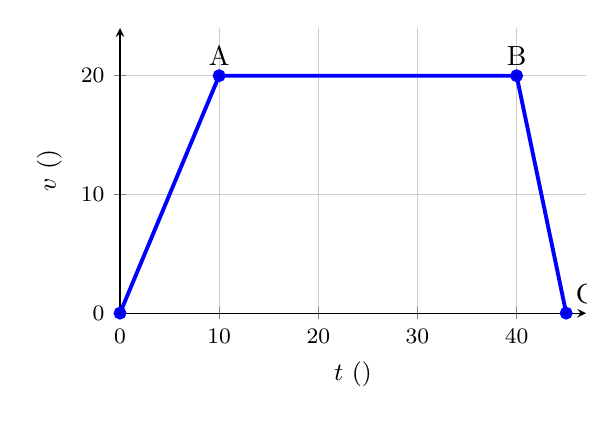
\begin{tikzpicture}
            \begin{axis}[grafica, xlabel={\(t\) (\unit{\s})}, ylabel={\(v\) (\unit{\m\per\s})}, xmin=0, xmax=47, ymin=0, ymax=24]
                \addplot coordinates {(0,0) (10,20) (40,20) (45,0)};
                \node[above] at (axis cs:10,20) {A}; \node[above] at (axis cs:40,20) {B}; \node[above right] at (axis cs:45,0) {C};
            \end{axis}
        \end{tikzpicture}
    \end{center}
    \textcolor{blue}{Tramo OA:} \(a = \frac{20 - 0}{10} = \textcolor{red}{\qty{2}{\m\per\square\s}}\) (acelerado). \textcolor{blue}{Tramo AB:} la velocidad no cambia: \(a = \textcolor{red}{0}\) (uniforme). \textcolor{blue}{Tramo BC:} \(a = \frac{0 - 20}{5} = \textcolor{red}{\qty{-4}{\m\per\square\s}}\) (retardado).
\end{example}

\begin{exercise}
    Explica la diferencia entre aceleración media y aceleración instantánea.
    \begin{solu}
        La \textcolor{red}{media} es la variación total de la velocidad dividida entre el tiempo total; la \textcolor{red}{instantánea}, la aceleración en un instante concreto. Coinciden si la aceleración es constante.
    \end{solu}
\end{exercise}

\begin{exercise}
    Un coche pasa de \qty{50}{\m\per\s} a \qty{65}{\m\per\s} en \qty{3}{\s}. ¿Cuál es su aceleración media?
    \begin{solu}
        \(a_m = \frac{65 - 50}{3} = \textcolor{red}{\qty{5}{\m\per\square\s}}\).
    \end{solu}
\end{exercise}

\begin{exercise}
    Un deportivo pasa de 0 a \qty{100}{\km\per\hour} en \qty{8.5}{\s}. ¿Qué aceleración media alcanza?
    \begin{solu}
        \(v = \frac{100}{\num{3.6}} = \qty{27.8}{\m\per\s}\); \(a_m = \frac{\num{27.8}}{\num{8.5}} = \textcolor{red}{\qty{3.27}{\m\per\square\s}}\).
    \end{solu}
\end{exercise}

\begin{exercise}
    El acelerador comunica a un coche una aceleración de \qty{3}{\m\per\square\s}. Si va a \qty{72}{\km\per\hour}, ¿cuánto tarda en alcanzar \qty{108}{\km\per\hour}?
    \begin{solu}
        \(v_0 = \qty{20}{\m\per\s}\); \(v = \qty{30}{\m\per\s}\); \(t = \frac{v - v_0}{a} = \frac{30 - 20}{3} = \textcolor{red}{\qty{3.3}{\s}}\).
    \end{solu}
\end{exercise}

\begin{exercise}
    Un automóvil circula a \qty{90}{\km\per\hour} y 10 s después su velocidad es \qty{108}{\km\per\hour}. ¿Cuál ha sido su aceleración?
    \begin{solu}
        \(v_0 = \qty{25}{\m\per\s}\); \(v = \qty{30}{\m\per\s}\); \(a = \frac{30 - 25}{10} = \textcolor{red}{\qty{0.5}{\m\per\square\s}}\).
    \end{solu}
\end{exercise}

\begin{exercise}
    Observa la gráfica y calcula la aceleración del móvil y su velocidad a los 8 s.
    \begin{center}
        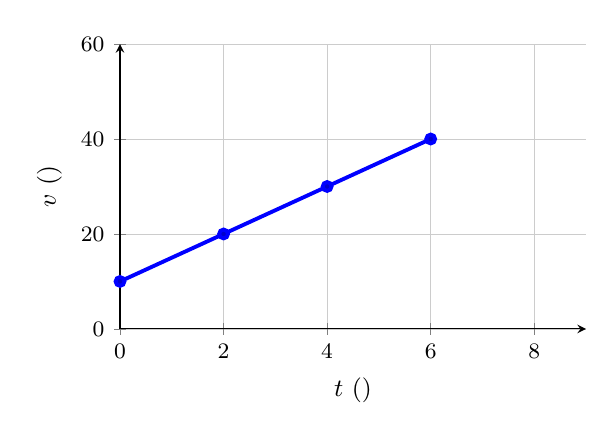
\begin{tikzpicture}
            \begin{axis}[grafica, xlabel={\(t\) (\unit{\s})}, ylabel={\(v\) (\unit{\m\per\s})}, xmin=0, xmax=9, ymin=0, ymax=60]
                \addplot coordinates {(0,10) (2,20) (4,30) (6,40)};
            \end{axis}
        \end{tikzpicture}
    \end{center}
    \begin{solu}
        La velocidad aumenta \qty{10}{\m\per\s} cada 2 s: \(a = \frac{40 - 10}{6} = \textcolor{red}{\qty{5}{\m\per\square\s}}\). A los 8 s: \(v = 10 + 5 \cdot 8 = \textcolor{red}{\qty{50}{\m\per\s}}\).
    \end{solu}
\end{exercise}

\begin{exercise}
    Un motorista que circula a \qty{90}{\km\per\hour} ve un obstáculo y detiene la moto en \qty{5}{\s}.
    \begin{enumerate}[label=\alph*)]
        \item ¿Cuál ha sido su aceleración?
        \item ¿Qué significa el signo del resultado?
    \end{enumerate}
    \begin{solu}
        a) \(a = \frac{0 - 25}{5} = \textcolor{red}{\qty{-5}{\m\per\square\s}}\). b) Que la velocidad \textcolor{red}{disminuye}: el movimiento es frenado y la aceleración tiene sentido contrario a la velocidad.
    \end{solu}
\end{exercise}

\begin{exercise}
    Un piloto de rally necesita 4 s para detener su coche, que va a \qty{108}{\km\per\hour}. ¿Cuál es su aceleración de frenado?
    \begin{solu}
        \(a = \frac{0 - 30}{4} = \textcolor{red}{\qty{-7.5}{\m\per\square\s}}\).
    \end{solu}
\end{exercise}

\begin{exercise}
    La tabla recoge la velocidad de un vehículo que acelera de forma constante. Complétala y calcula su aceleración.
    \begin{center}
        % --- tabla antigua ---
        % \begin{tblr}{colspec={lcccccc}, hlines, vlines, column{1}={bg=ocre!85, fg=white, font=\bfseries}}
            % \(v\) (\unit{\m\per\s}) & 3 & 6 & \ldots & 12 & \ldots & 18 \\
            % \(t\) (\unit{\s}) & 1 & 2 & 3 & 4 & 5 & 6 \\
        % \end{tblr}
        % --- tabla nueva ---
        \begin{tabular}{@{}lcccccc@{}}
            \toprule
            \textbf{\(v\) (\unit{\m\per\s})} & 3 & 6 & \ldots & 12 & \ldots & 18 \\[3pt]
            \textbf{\(t\) (\unit{\s})} & 1 & 2 & 3 & 4 & 5 & 6 \\
            \bottomrule
        \end{tabular}
    \end{center}
    \begin{solu}
        La velocidad aumenta \qty{3}{\m\per\s} cada segundo: \(a = \textcolor{red}{\qty{3}{\m\per\square\s}}\). Los valores que faltan son \textcolor{red}{9} y \textcolor{red}{\qty{15}{\m\per\s}}.
    \end{solu}
\end{exercise}

%========================================================================================
\section{Movimiento rectilíneo y uniforme (MRU)}
%========================================================================================

El \textbf{movimiento rectilíneo y uniforme} (MRU) tiene:
\begin{itemize}
    \item trayectoria \textbf{rectilínea};
    \item velocidad \textbf{constante} en módulo, dirección y sentido;
    \item aceleración \textbf{nula}.
\end{itemize}

\subsection{Ecuaciones y gráficas del MRU}

La tabla recoge las posiciones de un móvil:
\begin{center}
    % --- tabla antigua ---
    % \begin{tblr}{colspec={lccccc}, hlines, vlines, column{1}={bg=ocre!85, fg=white, font=\bfseries}}
        % \(s\) (\unit{\m}) & 0 & 10 & 20 & 50 & 100 \\
        % \(t\) (\unit{\s}) & 0 & 1 & 2 & 5 & 10 \\
    % \end{tblr}
    % --- tabla nueva ---
    \begin{tabular}{@{}lccccc@{}}
        \toprule
        \textbf{\(s\) (\unit{\m})} & 0 & 10 & 20 & 50 & 100 \\[3pt]
        \textbf{\(t\) (\unit{\s})} & 0 & 1 & 2 & 5 & 10 \\
        \bottomrule
    \end{tabular}
\end{center}
Recorre espacios iguales en tiempos iguales: \qty{10}{\m} cada segundo. Su gráfica \(s\)-\(t\) es una \textbf{recta} cuya \textbf{pendiente} es la velocidad, \(v = \frac{100}{10} = \qty{10}{\m\per\s}\), y su gráfica \(v\)-\(t\) es una recta horizontal.

\begin{center}
    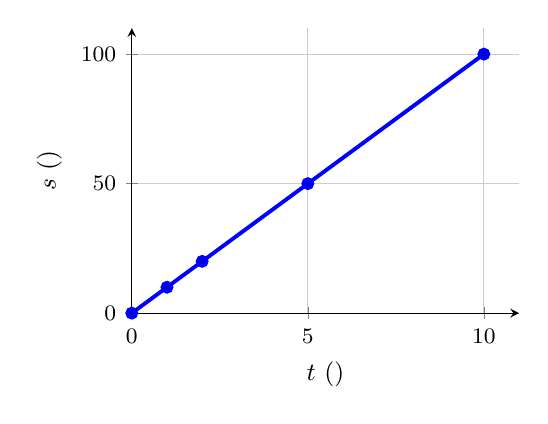
\begin{tikzpicture}
        \begin{axis}[grafica, width=6.5cm, xlabel={\(t\) (\unit{\s})}, ylabel={\(s\) (\unit{\m})}, xmin=0, xmax=11, ymin=0, ymax=110]
            \addplot coordinates {(0,0) (1,10) (2,20) (5,50) (10,100)};
        \end{axis}
    \end{tikzpicture}
    \qquad
    \begin{tikzpicture}
        \begin{axis}[grafica, width=6.5cm, xlabel={\(t\) (\unit{\s})}, ylabel={\(v\) (\unit{\m\per\s})}, xmin=0, xmax=11, ymin=0, ymax=12]
            \addplot[mark=none] coordinates {(0,10) (10,10)};
        \end{axis}
    \end{tikzpicture}
\end{center}

\begin{centeredequation}
    s = s_0 + v \cdot t
\end{centeredequation}
donde \(s_0\) es la posición inicial (si el móvil parte del origen, \(s = v \cdot t\)).

\begin{example}
    \textbf{Dos móviles que se cruzan.} Un coche A sale del origen a \qty{20}{\m\per\s} y, a la vez, un coche B sale de un punto situado a \qty{700}{\m} y va a su encuentro a \qty{15}{\m\per\s}. ¿Cuándo y dónde se cruzan?

    \textcolor{blue}{Ecuaciones} (tomando positivo el sentido de A): \(s_A = 20\,t\); \quad \(s_B = 700 - 15\,t\).

    \textcolor{blue}{Se cruzan cuando están en la misma posición:} \(20\,t = 700 - 15\,t \;\Rightarrow\; 35\,t = 700 \;\Rightarrow\; t = \textcolor{red}{\qty{20}{\s}}\); \(s = 20 \cdot 20 = \textcolor{red}{\qty{400}{\m}}\) del origen. A ha recorrido \qty{400}{\m} y B, \qty{300}{\m}. En la gráfica \(s\)-\(t\), el punto de corte de las dos rectas indica dónde y cuándo se cruzan:
    \begin{center}
        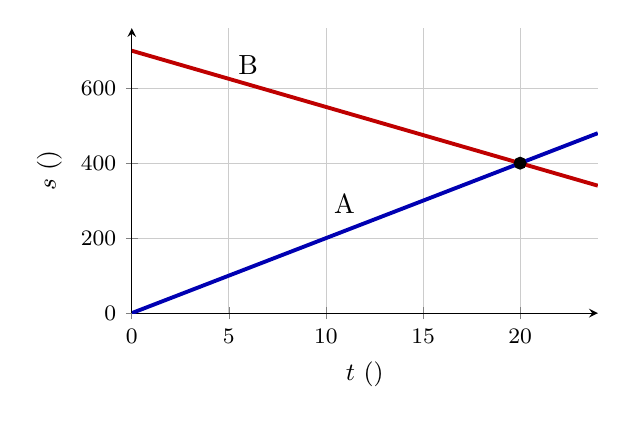
\begin{tikzpicture}
            \begin{axis}[grafica, xlabel={\(t\) (\unit{\s})}, ylabel={\(s\) (\unit{\m})}, xmin=0, xmax=24, ymin=0, ymax=760]
                \addplot[mark=none, color=blue!70!black] coordinates {(0,0) (24,480)}; \node[above left] at (axis cs:12,240) {A};
                \addplot[mark=none] coordinates {(0,700) (24,340)}; \node[above] at (axis cs:6,610) {B};
                \addplot[only marks, mark=*, color=black] coordinates {(20,400)};
            \end{axis}
        \end{tikzpicture}
    \end{center}
\end{example}

\begin{exercise}
    Un guepardo sigue una trayectoria rectilínea durante 8 s a \qty{108}{\km\per\hour} constantes. ¿Qué espacio recorre?
    \begin{solu}
        \(v = \qty{30}{\m\per\s}\); \(s = v \cdot t = 30 \cdot 8 = \textcolor{red}{\qty{240}{\m}}\).
    \end{solu}
\end{exercise}

\begin{exercise}
    La gráfica muestra el movimiento de dos cuerpos A y B. ¿En qué instante y en qué posición se cruzan? ¿Qué velocidad lleva cada uno?
    \begin{center}
        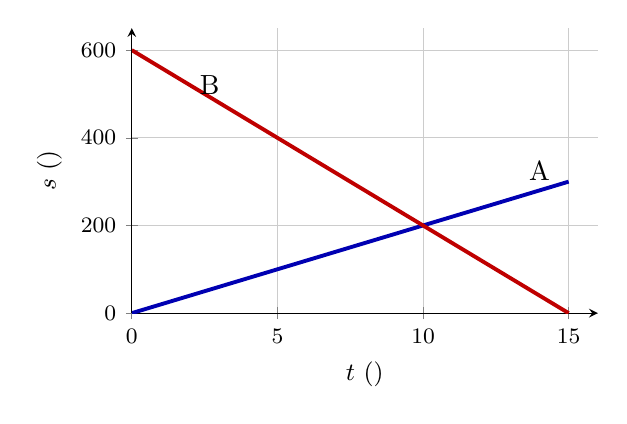
\begin{tikzpicture}
            \begin{axis}[grafica, xlabel={\(t\) (\unit{\s})}, ylabel={\(s\) (\unit{\m})}, xmin=0, xmax=16, ymin=0, ymax=650]
                \addplot[mark=none, color=blue!70!black] coordinates {(0,0) (15,300)}; \node[above] at (axis cs:14,280) {A};
                \addplot[mark=none] coordinates {(0,600) (15,0)}; \node[right] at (axis cs:2,520) {B};
            \end{axis}
        \end{tikzpicture}
    \end{center}
    \begin{solu}
        \(v_A = \frac{300}{15} = \textcolor{red}{\qty{20}{\m\per\s}}\); \(v_B = \frac{0 - 600}{15} = \textcolor{red}{\qty{-40}{\m\per\s}}\) (se mueve hacia el origen).
        \(20\,t = 600 - 40\,t \Rightarrow t = \textcolor{red}{\qty{10}{\s}}\), en \(s = \textcolor{red}{\qty{200}{\m}}\).
    \end{solu}
\end{exercise}

\begin{exercise}
    Dos vehículos parten a la vez del mismo punto a \qty{80}{\m\per\s} y \qty{70}{\m\per\s}. ¿Qué distancia los separa al cabo de 5 s si
    \begin{enumerate}[label=\alph*)]
        \item circulan en el mismo sentido;
        \item circulan en sentidos contrarios?
    \end{enumerate}
    \begin{solu}
        Recorren \(80 \cdot 5 = \qty{400}{\m}\) y \(70 \cdot 5 = \qty{350}{\m}\).
        a) \(400 - 350 = \textcolor{red}{\qty{50}{\m}}\). b) \(400 + 350 = \textcolor{red}{\qty{750}{\m}}\).
    \end{solu}
\end{exercise}

\begin{exercise}
    La tabla recoge las posiciones de un móvil:
    \begin{center}
        % --- tabla antigua ---
        % \begin{tblr}{colspec={lccccc}, hlines, vlines, column{1}={bg=ocre!85, fg=white, font=\bfseries}}
            % \(s\) (\unit{\m}) & 2 & 14 & 32 & 44 & 68 \\
            % \(t\) (\unit{\s}) & 0 & 2 & 5 & 7 & 11 \\
        % \end{tblr}
        % --- tabla nueva ---
        \begin{tabular}{@{}lccccc@{}}
            \toprule
            \textbf{\(s\) (\unit{\m})} & 2 & 14 & 32 & 44 & 68 \\[3pt]
            \textbf{\(t\) (\unit{\s})} & 0 & 2 & 5 & 7 & 11 \\
            \bottomrule
        \end{tabular}
    \end{center}
    \begin{enumerate}[label=\alph*)]
        \item Represéntalos y clasifica el movimiento.
        \item Halla la velocidad y escribe la ecuación del movimiento.
        \item ¿Cuánto tarda en recorrer \qty{100}{\m}?
    \end{enumerate}
    \begin{solu}
        a) Los puntos están sobre una recta: es un \textcolor{red}{MRU}.
        b) \(v = \frac{68 - 2}{11} = \textcolor{red}{\qty{6}{\m\per\s}}\); \(s = 2 + 6\,t\).
        c) \(t = \frac{100}{6} = \textcolor{red}{\qty{16.7}{\s}}\).
    \end{solu}
\end{exercise}

\begin{exercise}
    La gráfica \(v\)-\(t\) de un móvil es una recta horizontal en \(v = \qty{8}{\m\per\s}\). ¿Cuánto tarda en recorrer \qty{120}{\m}?
    \begin{solu}
        Es un MRU: \(t = \frac{s}{v} = \frac{120}{8} = \textcolor{red}{\qty{15}{\s}}\).
    \end{solu}
\end{exercise}

\begin{exercise}
    Dos coches, A y B, salen a la vez uno al encuentro del otro desde dos puntos separados \qty{2}{\km}. A va a \qty{54}{\km\per\hour} y B a \qty{90}{\km\per\hour}. ¿Cuánto tardan en encontrarse y dónde?
    \begin{solu}
        \(v_A = \qty{15}{\m\per\s}\); \(v_B = \qty{25}{\m\per\s}\). \(15\,t = 2000 - 25\,t \Rightarrow t = \textcolor{red}{\qty{50}{\s}}\); se encuentran a \(15 \cdot 50 = \textcolor{red}{\qty{750}{\m}}\) del punto de salida de A.
    \end{solu}
\end{exercise}

\begin{exercise}
    Un viajero pierde el barco, que salió hace 1 h y navega a \qty{30}{\km\per\hour}. Contrata una lancha que navega a \qty{50}{\km\per\hour}.
    \begin{enumerate}[label=\alph*)]
        \item ¿Cuánto tarda en alcanzarlo?
        \item ¿A qué distancia de la costa?
    \end{enumerate}
    \begin{solu}
        Cuando salga la lancha, el barco estará a \qty{30}{\km}. \(50\,t = 30 + 30\,t \Rightarrow t = \textcolor{red}{\qty{1.5}{\hour}}\). Distancia: \(50 \cdot \num{1.5} = \textcolor{red}{\qty{75}{\km}}\).
    \end{solu}
\end{exercise}

\begin{exercise}
    Un coche sale a las 9:00 a \qty{20}{\m\per\s}. A las 9:20 sale del mismo punto otro a \qty{30}{\m\per\s} para alcanzarlo. ¿A qué hora y a qué distancia lo alcanza?
    \begin{solu}
        En 20 min (\qty{1200}{\s}) el primero ha recorrido \(20 \cdot 1200 = \qty{24000}{\m}\). Contando el tiempo desde las 9:20: \(30\,t = 24000 + 20\,t \Rightarrow t = \qty{2400}{\s} = \qty{40}{\minute}\). Lo alcanza a las \textcolor{red}{10:00}, a \(30 \cdot 2400 = \qty{72000}{\m} = \textcolor{red}{\qty{72}{\km}}\).
    \end{solu}
\end{exercise}

%========================================================================================
\section{Movimiento rectilíneo uniformemente variado (MRUV)}
%========================================================================================

Un cuerpo describe un \textbf{movimiento rectilíneo uniformemente variado} (MRUV) si su trayectoria es rectilínea y su \textbf{aceleración es constante}. Puede ser:
\begin{itemize}
    \item \textbf{acelerado} (MRUA), si la aceleración es positiva (la velocidad aumenta);
    \item \textbf{retardado} o frenado (MRUR), si la aceleración es negativa (la velocidad disminuye).
\end{itemize}

\subsection{Ecuaciones del MRUV}

\begin{center}
    % --- tabla antigua ---
    % \begin{tblr}{colspec={lccccc}, hlines, vlines, column{1}={bg=ocre!85, fg=white, font=\bfseries}}
        % \(v\) (\unit{\m\per\s}) & 2 & 3 & 4 & 5 & 6 \\
        % \(t\) (\unit{\s}) & 0 & 1 & 2 & 3 & 4 \\
    % \end{tblr}
    % --- tabla nueva ---
    \begin{tabular}{@{}lccccc@{}}
        \toprule
        \textbf{\(v\) (\unit{\m\per\s})} & 2 & 3 & 4 & 5 & 6 \\[3pt]
        \textbf{\(t\) (\unit{\s})} & 0 & 1 & 2 & 3 & 4 \\
        \bottomrule
    \end{tabular}
    \qquad
    % --- tabla antigua ---
    % \begin{tblr}{colspec={lccccccc}, hlines, vlines, column{1}={bg=ocre!85, fg=white, font=\bfseries}}
        % \(s\) (\unit{\m}) & 0 & \num{2.5} & 6 & \num{10.5} & 16 & \num{22.5} & 30 \\
        % \(t\) (\unit{\s}) & 0 & 1 & 2 & 3 & 4 & 5 & 6 \\
    % \end{tblr}
    % --- tabla nueva ---
    \begin{tabular}{@{}lccccccc@{}}
        \toprule
        \textbf{\(s\) (\unit{\m})} & 0 & \num{2.5} & 6 & \num{10.5} & 16 & \num{22.5} & 30 \\[3pt]
        \textbf{\(t\) (\unit{\s})} & 0 & 1 & 2 & 3 & 4 & 5 & 6 \\
        \bottomrule
    \end{tabular}
\end{center}

La gráfica \(v\)-\(t\) de un MRUA es una \textbf{recta} cuya pendiente es la aceleración (aquí \(a = \qty{1}{\m\per\square\s}\)) y que corta el eje vertical en la velocidad inicial (\(v_0 = \qty{2}{\m\per\s}\)). La gráfica \(s\)-\(t\) es una \textbf{parábola}: el espacio no es proporcional al tiempo.

\begin{center}
    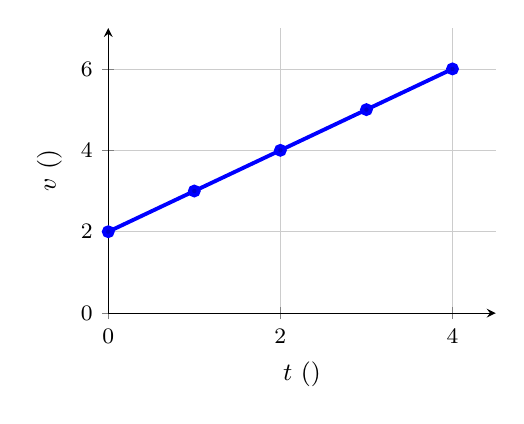
\begin{tikzpicture}
        \begin{axis}[grafica, width=6.5cm, xlabel={\(t\) (\unit{\s})}, ylabel={\(v\) (\unit{\m\per\s})}, xmin=0, xmax=4.5, ymin=0, ymax=7]
            \addplot coordinates {(0,2) (1,3) (2,4) (3,5) (4,6)};
        \end{axis}
    \end{tikzpicture}
    \qquad
    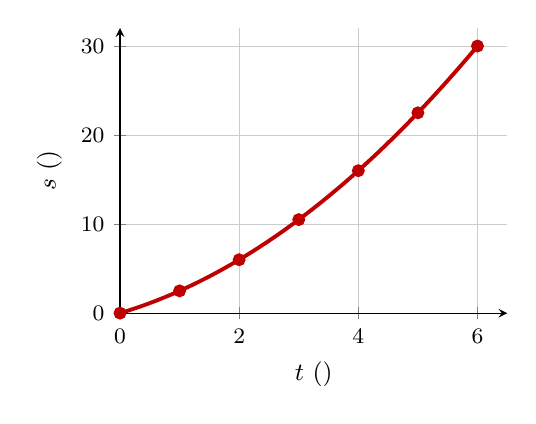
\begin{tikzpicture}
        \begin{axis}[grafica, width=6.5cm, xlabel={\(t\) (\unit{\s})}, ylabel={\(s\) (\unit{\m})}, xmin=0, xmax=6.5, ymin=0, ymax=32]
            \addplot[mark=none, domain=0:6, samples=40] {2*x + 0.5*x^2};
            \addplot[only marks] coordinates {(0,0) (1,2.5) (2,6) (3,10.5) (4,16) (5,22.5) (6,30)};
        \end{axis}
    \end{tikzpicture}
\end{center}

Las ecuaciones del MRUV son:
\begin{centeredequation}
    v = v_0 + a \cdot t \qquad\qquad s = s_0 + v_0 \cdot t + \frac{1}{2}\, a \cdot t^2
\end{centeredequation}
En un MRUR se usan las mismas ecuaciones, con \(a\) negativa. Si el móvil parte del reposo y del origen: \(v = a \cdot t\) y \(s = \frac{1}{2}\, a \cdot t^2\).

\begin{remark}
    \textbf{Una ecuación útil.} Despejando el tiempo de la primera ecuación y sustituyéndolo en la segunda se obtiene una relación que no depende del tiempo: \(v^2 - v_0^2 = 2\,a\,(s - s_0)\). Es muy práctica para calcular distancias de frenado.
\end{remark}

\begin{example}
    Un vehículo que circula a \qty{10}{\m\per\s} acelera durante 10 s hasta \qty{20}{\m\per\s}. Calcula su aceleración y el espacio recorrido.
    \[ a = \frac{20 - 10}{10} = \textcolor{red}{\qty{1}{\m\per\square\s}}; \qquad s = 10 \cdot 10 + \frac{1}{2} \cdot 1 \cdot 10^2 = \textcolor{red}{\qty{150}{\m}} \]
\end{example}

\begin{example}
    Un conductor que va a \qty{30}{\m\per\s} ve un desprendimiento de rocas y frena hasta detenerse en 12 s. Calcula la aceleración de frenado y el espacio que recorre hasta pararse.
    \[ 0 = 30 + a \cdot 12 \Rightarrow a = \textcolor{red}{\qty{-2.5}{\m\per\square\s}}; \qquad s = 30 \cdot 12 - \frac{1}{2} \cdot \num{2.5} \cdot 12^2 = 360 - 180 = \textcolor{red}{\qty{180}{\m}} \]
\end{example}

\begin{remark}
    \textbf{La distancia de seguridad.} Para evitar accidentes hay que guardar una \textbf{distancia de seguridad} (o de parada) con el vehículo de delante. Incluye el espacio recorrido durante el \textbf{tiempo de reacción} (lo que tardamos en pisar el freno, en el que el coche sigue a velocidad constante) y el espacio de frenado.
\end{remark}

\begin{exercise}
    El maquinista de un tren que circula a \qty{90}{\km\per\hour} ve un obstáculo en la vía a \qty{120}{\m} y frena con una aceleración de \qty{3}{\m\per\square\s}. ¿Se detendrá antes de llegar al obstáculo?
    \begin{solu}
        \(v_0 = \qty{25}{\m\per\s}\). Con \(v^2 - v_0^2 = 2\,a\,s\): \(0 - 625 = 2 \cdot (-3) \cdot s \Rightarrow s = \textcolor{red}{\qty{104.2}{\m}}\). \textcolor{red}{Sí} se detiene, a unos \qty{16}{\m} del obstáculo.
    \end{solu}
\end{exercise}

\begin{exercise}
    Describe el movimiento en cada tramo de la gráfica y calcula el espacio recorrido en el tramo AB.
    \begin{center}
        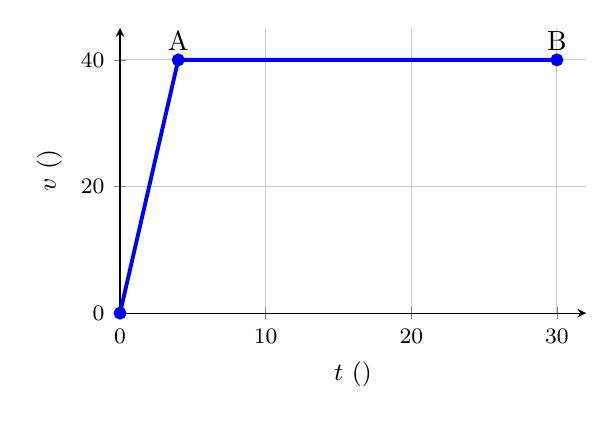
\begin{tikzpicture}
            \begin{axis}[grafica, xlabel={\(t\) (\unit{\s})}, ylabel={\(v\) (\unit{\m\per\s})}, xmin=0, xmax=32, ymin=0, ymax=45]
                \addplot coordinates {(0,0) (4,40) (30,40)};
                \node[above] at (axis cs:4,40) {A}; \node[above] at (axis cs:30,40) {B};
            \end{axis}
        \end{tikzpicture}
    \end{center}
    \begin{solu}
        Tramo OA: \textcolor{red}{MRUA}, \(a = \frac{40}{4} = \qty{10}{\m\per\square\s}\). Tramo AB: \textcolor{red}{MRU} a \qty{40}{\m\per\s}. Espacio en AB: \(s = 40 \cdot (30 - 4) = \textcolor{red}{\qty{1040}{\m}}\).
    \end{solu}
\end{exercise}

\begin{exercise}
    Un conductor que circula a \qty{72}{\km\per\hour} ve un obstáculo y frena de manera uniforme hasta detenerse en 4 s. Calcula el espacio que recorre hasta pararse:
    \begin{enumerate}[label=\alph*)]
        \item sin tener en cuenta el tiempo de reacción;
        \item si su tiempo de reacción es de 2 s.
    \end{enumerate}
    \begin{solu}
        \(v_0 = \qty{20}{\m\per\s}\); \(a = \frac{0 - 20}{4} = \qty{-5}{\m\per\square\s}\).
        a) \(s = 20 \cdot 4 - \frac{1}{2} \cdot 5 \cdot 4^2 = \textcolor{red}{\qty{40}{\m}}\).
        b) Durante la reacción recorre \(20 \cdot 2 = \qty{40}{\m}\) a velocidad constante: en total, \textcolor{red}{\qty{80}{\m}}.
    \end{solu}
\end{exercise}

\begin{exercise}
    Una ciclista que va a \qty{36}{\km\per\hour} frena con una aceleración de \qty{1}{\m\per\square\s} durante 4 s.
    \begin{enumerate}[label=\alph*)]
        \item ¿Qué velocidad lleva al cabo de los 4 s?
        \item ¿Qué espacio ha recorrido mientras frenaba?
    \end{enumerate}
    \begin{solu}
        \(v_0 = \qty{10}{\m\per\s}\); \(a = \qty{-1}{\m\per\square\s}\).
        a) \(v = 10 - 1 \cdot 4 = \textcolor{red}{\qty{6}{\m\per\s}}\). b) \(s = 10 \cdot 4 - \frac{1}{2} \cdot 1 \cdot 4^2 = \textcolor{red}{\qty{32}{\m}}\).
    \end{solu}
\end{exercise}

\begin{exercise}
    Un avión toma tierra a \qty{216}{\km\per\hour} y frena de manera uniforme usando toda la pista, de \qty{1800}{\m}.
    \begin{enumerate}[label=\alph*)]
        \item ¿Cuál es su aceleración de frenado?
        \item ¿Cuánto tarda en detenerse?
        \item ¿Qué pasaría si otro avión aterrizara a \qty{252}{\km\per\hour} con la misma aceleración?
    \end{enumerate}
    \begin{solu}
        \(v_0 = \qty{60}{\m\per\s}\).
        a) \(0 - 60^2 = 2\,a \cdot 1800 \Rightarrow a = \textcolor{red}{\qty{-1}{\m\per\square\s}}\).
        b) \(t = \frac{0 - 60}{-1} = \textcolor{red}{\qty{60}{\s}}\).
        c) Con \(v_0 = \qty{70}{\m\per\s}\): \(s = \frac{70^2}{2} = \qty{2450}{\m}\). \textcolor{red}{Necesitaría más pista} de la que hay: se saldría de ella.
    \end{solu}
\end{exercise}

\begin{exercise}
    Un vehículo parte del reposo con una aceleración de \qty{2.5}{\m\per\square\s}.
    \begin{enumerate}[label=\alph*)]
        \item ¿Qué velocidad tiene a los 8 s? ¿Qué espacio ha recorrido?
        \item Después sigue 3 minutos a esa velocidad. ¿Qué espacio recorre?
        \item Por último, frena hasta detenerse en 4 s. ¿Cuál es su aceleración de frenado y qué espacio recorre?
    \end{enumerate}
    \begin{solu}
        a) \(v = \num{2.5} \cdot 8 = \textcolor{red}{\qty{20}{\m\per\s}}\); \(s = \frac{1}{2} \cdot \num{2.5} \cdot 8^2 = \textcolor{red}{\qty{80}{\m}}\).
        b) MRU: \(s = 20 \cdot 180 = \textcolor{red}{\qty{3600}{\m}}\).
        c) \(a = \frac{0 - 20}{4} = \textcolor{red}{\qty{-5}{\m\per\square\s}}\); \(s = 20 \cdot 4 - \frac{1}{2} \cdot 5 \cdot 4^2 = \textcolor{red}{\qty{40}{\m}}\).
    \end{solu}
\end{exercise}

\begin{exercise}
    Esta gráfica corresponde a un MRUA. ¿Cuál es la velocidad inicial? ¿Y la aceleración? ¿Qué espacio recorre el móvil en el primer segundo? ¿Y en el segundo siguiente?
    \begin{center}
        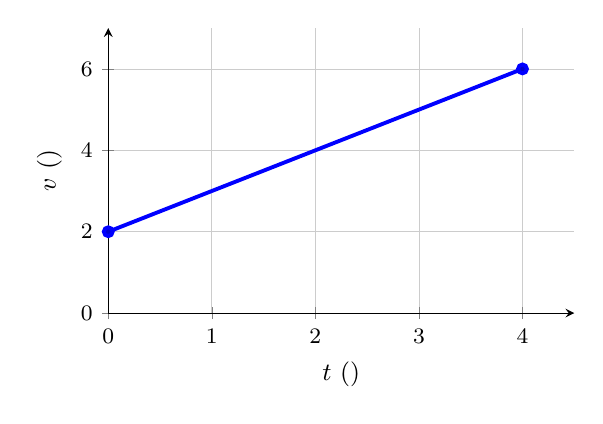
\begin{tikzpicture}
            \begin{axis}[grafica, xlabel={\(t\) (\unit{\s})}, ylabel={\(v\) (\unit{\m\per\s})}, xmin=0, xmax=4.5, ymin=0, ymax=7]
                \addplot coordinates {(0,2) (4,6)};
            \end{axis}
        \end{tikzpicture}
    \end{center}
    \begin{solu}
        \(v_0 = \textcolor{red}{\qty{2}{\m\per\s}}\); \(a = \frac{6 - 2}{4} = \textcolor{red}{\qty{1}{\m\per\square\s}}\). Con \(s = 2t + \frac{1}{2}t^2\): \(s(1) = \qty{2.5}{\m}\) y \(s(2) = \qty{6}{\m}\). En el primer segundo recorre \textcolor{red}{\qty{2.5}{\m}} y en el segundo, \(6 - \num{2.5} = \textcolor{red}{\qty{3.5}{\m}}\).
    \end{solu}
\end{exercise}

\begin{exercise}
    Calcula la aceleración en cada tramo de esta gráfica:
    \begin{center}
        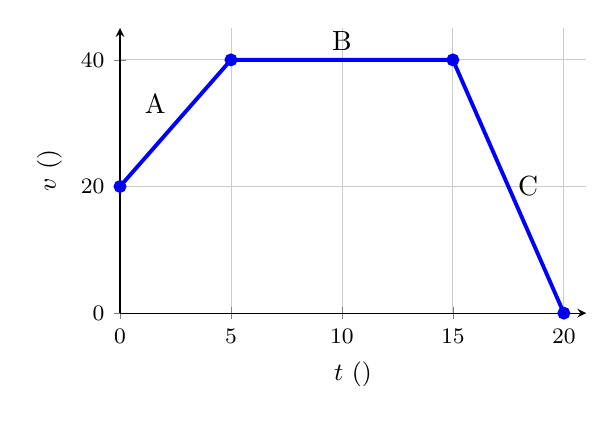
\begin{tikzpicture}
            \begin{axis}[grafica, xlabel={\(t\) (\unit{\s})}, ylabel={\(v\) (\unit{\m\per\s})}, xmin=0, xmax=21, ymin=0, ymax=45]
                \addplot coordinates {(0,20) (5,40) (15,40) (20,0)};
                \node[above left] at (axis cs:2.5,30) {A}; \node[above] at (axis cs:10,40) {B}; \node[right] at (axis cs:17.5,20) {C};
            \end{axis}
        \end{tikzpicture}
    \end{center}
    \begin{solu}
        A: \(a = \frac{40 - 20}{5} = \textcolor{red}{\qty{4}{\m\per\square\s}}\). B: \(a = \textcolor{red}{0}\). C: \(a = \frac{0 - 40}{5} = \textcolor{red}{\qty{-8}{\m\per\square\s}}\).
    \end{solu}
\end{exercise}

\begin{exercise}
    La conductora de un coche que va por una autopista a \qty{108}{\km\per\hour} frena y se detiene en 6 s. ¿Qué espacio recorre hasta detenerse?
    \begin{solu}
        \(a = \frac{0 - 30}{6} = \qty{-5}{\m\per\square\s}\); \(s = 30 \cdot 6 - \frac{1}{2} \cdot 5 \cdot 36 = \textcolor{red}{\qty{90}{\m}}\).
    \end{solu}
\end{exercise}

\begin{exercise}
    Un avión necesita alcanzar \qty{252}{\km\per\hour} para despegar. Si parte del reposo y tarda 50 s:
    \begin{enumerate}[label=\alph*)]
        \item ¿qué aceleración (constante) le dan los motores?
        \item ¿qué longitud mínima debe tener la pista?
    \end{enumerate}
    \begin{solu}
        \(v = \qty{70}{\m\per\s}\). a) \(a = \frac{70}{50} = \textcolor{red}{\qty{1.4}{\m\per\square\s}}\). b) \(s = \frac{1}{2} \cdot \num{1.4} \cdot 50^2 = \textcolor{red}{\qty{1750}{\m}}\).
    \end{solu}
\end{exercise}

\begin{exercise}
    Calcula la posición y la velocidad a los 4 s de estos movimientos:
    \begin{enumerate}[label=\alph*)]
        \item posición inicial \qty{20}{\m}, velocidad inicial \qty{12}{\m\per\s} y aceleración \qty{-3}{\m\per\square\s};
        \item parte del reposo desde el origen con una aceleración de \qty{3}{\m\per\square\s}.
    \end{enumerate}
    \begin{solu}
        a) \(s = 20 + 12 \cdot 4 - \frac{1}{2} \cdot 3 \cdot 16 = \textcolor{red}{\qty{44}{\m}}\); \(v = 12 - 3 \cdot 4 = \textcolor{red}{0}\) (está parado en ese instante).
        b) \(s = \frac{1}{2} \cdot 3 \cdot 16 = \textcolor{red}{\qty{24}{\m}}\); \(v = 3 \cdot 4 = \textcolor{red}{\qty{12}{\m\per\s}}\).
    \end{solu}
\end{exercise}

\begin{exercise}
    Un tren que va a \qty{54}{\km\per\hour} recorre \qty{90}{\m} desde que empieza a frenar hasta que se para. Si la aceleración es constante, calcula su valor y el tiempo de frenado.
    \begin{solu}
        \(v_0 = \qty{15}{\m\per\s}\). \(0 - 15^2 = 2\,a \cdot 90 \Rightarrow a = \textcolor{red}{\qty{-1.25}{\m\per\square\s}}\); \(t = \frac{0 - 15}{\num{-1.25}} = \textcolor{red}{\qty{12}{\s}}\).
    \end{solu}
\end{exercise}

%========================================================================================
\section{Movimientos verticales: caída libre y lanzamiento vertical}
%========================================================================================

En el siglo \textsc{xvii}, \textbf{Galileo Galilei} demostró que, si se desprecia la resistencia del aire, todos los cuerpos caen hacia la Tierra con la misma aceleración, independientemente de su masa: la \textbf{aceleración de la gravedad}, \(g = \qty{9.8}{\m\per\square\s}\).

\subsection{Caída libre}

Un cuerpo que se deja caer desde el reposo describe un \textbf{MRUA} con \(v_0 = 0\) y \(a = g\). Tomando como origen el punto desde el que cae y el sentido positivo hacia abajo:
\begin{centeredequation*}
    v = g \cdot t \qquad\qquad s = \frac{1}{2}\, g \cdot t^2
\end{centeredequation*}

\begin{example}
    La Torre de Pisa mide unos \qty{56}{\m}. ¿Cuánto tarda en llegar al suelo un objeto que se deja caer desde lo alto? ¿Con qué velocidad llega?
    \[ 56 = \frac{1}{2} \cdot \num{9.8} \cdot t^2 \Rightarrow t = \sqrt{\frac{2 \cdot 56}{\num{9.8}}} = \textcolor{red}{\qty{3.38}{\s}}; \qquad v = \num{9.8} \cdot \num{3.38} = \textcolor{red}{\qty{33.1}{\m\per\s}} \]
\end{example}

\subsection{Lanzamiento vertical hacia abajo}

Es un MRUA con velocidad inicial \(v_0\) hacia abajo y aceleración \(g\):
\begin{centeredequation*}
    v = v_0 + g \cdot t \qquad\qquad s = v_0 \cdot t + \frac{1}{2}\, g \cdot t^2
\end{centeredequation*}

\begin{example}
    Desde \qty{45}{\m} de altura se lanza un objeto hacia abajo a \qty{3}{\m\per\s}. ¿Cuánto tarda en llegar al suelo y con qué velocidad?
    \[ 45 = 3\,t + \num{4.9}\,t^2 \Rightarrow \num{4.9}\,t^2 + 3\,t - 45 = 0 \Rightarrow t = \frac{-3 + \sqrt{9 + 4 \cdot \num{4.9} \cdot 45}}{2 \cdot \num{4.9}} = \textcolor{red}{\qty{2.74}{\s}} \]
    (La otra solución es negativa y no tiene sentido físico.) \quad \(v = 3 + \num{9.8} \cdot \num{2.74} = \textcolor{red}{\qty{29.9}{\m\per\s}}\).
\end{example}

\subsection{Lanzamiento vertical hacia arriba}

Un cuerpo lanzado hacia arriba con velocidad \(v_0\) describe un \textbf{MRUR}: la gravedad tiene sentido contrario al movimiento y la velocidad disminuye hasta anularse en el punto más alto. Después el cuerpo cae en caída libre. Tomando el sentido positivo hacia arriba:
\begin{centeredequation*}
    v = v_0 - g \cdot t \qquad\qquad y = v_0 \cdot t - \frac{1}{2}\, g \cdot t^2
\end{centeredequation*}
El tiempo de subida es igual al de bajada y, en cada punto, el módulo de la velocidad es el mismo al subir y al bajar (figura~\ref{fig:lanzamiento_vertical}).

\begin{figure}[H]
    \centering
    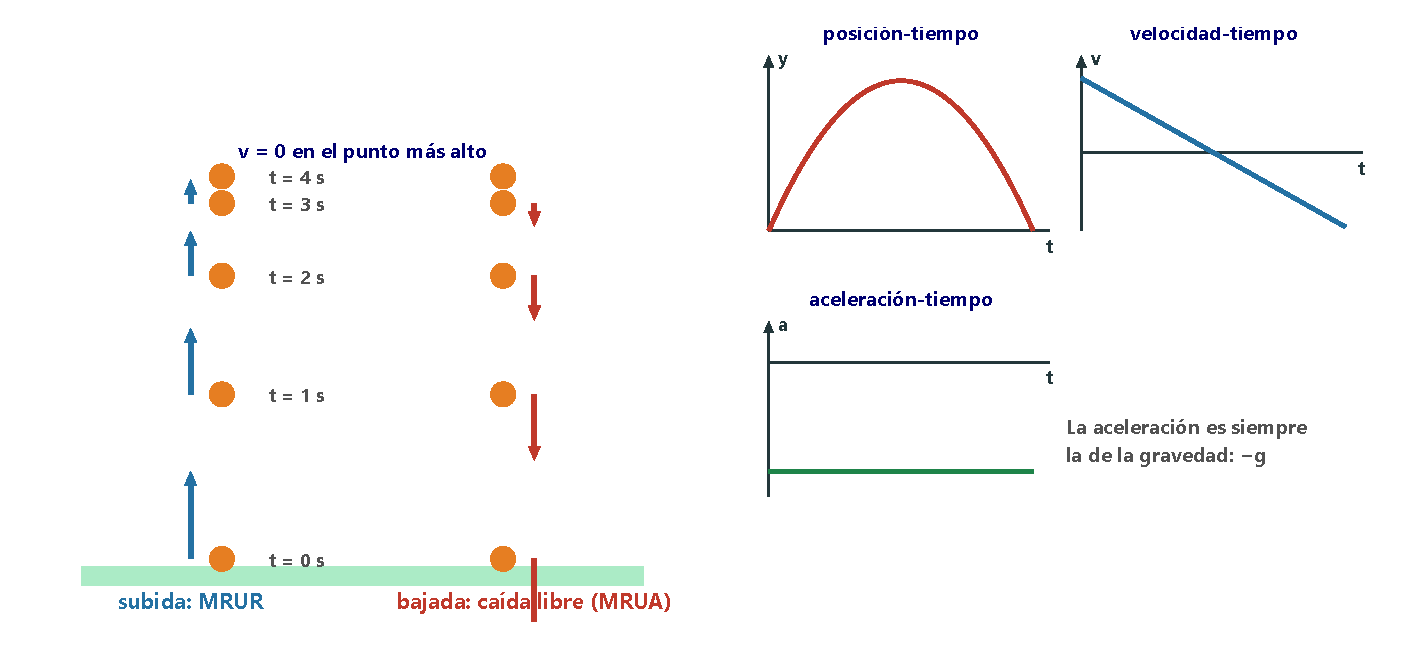
\includegraphics[width=0.95\textwidth]{images/UD7/lanzamiento_vertical}
    \caption{Lanzamiento vertical hacia arriba (\(v_0 = \qty{40}{\m\per\s}\)) y gráficas posición-tiempo, velocidad-tiempo y aceleración-tiempo.}
    \label{fig:lanzamiento_vertical}
\end{figure}

\begin{example}
    Se lanza una pelota hacia arriba a \qty{29.4}{\m\per\s}. Calcula: a) el tiempo que tarda en llegar al punto más alto; b) la altura máxima; c) cuándo pasa por \qty{40}{\m} de altura.

    a) En el punto más alto \(v = 0\): \(0 = \num{29.4} - \num{9.8}\,t \Rightarrow t = \textcolor{red}{\qty{3}{\s}}\).

    b) \(y = \num{29.4} \cdot 3 - \num{4.9} \cdot 3^2 = \textcolor{red}{\qty{44.1}{\m}}\).

    c) \(40 = \num{29.4}\,t - \num{4.9}\,t^2 \Rightarrow \num{4.9}\,t^2 - \num{29.4}\,t + 40 = 0 \Rightarrow t = \dfrac{\num{29.4} \pm \sqrt{\num{29.4}^2 - 4 \cdot \num{4.9} \cdot 40}}{2 \cdot \num{4.9}}\): \(t_1 = \textcolor{red}{\qty{2.09}{\s}}\) (al subir) y \(t_2 = \textcolor{red}{\qty{3.91}{\s}}\) (al bajar). En total tarda \qty{6}{\s} en volver al suelo.
\end{example}

\begin{exercise}
    Desde un edificio en construcción, a \qty{45}{\m} del suelo, se cae un ladrillo.
    \begin{enumerate}[label=\alph*)]
        \item ¿Cuánto tarda en llegar al suelo?
        \item ¿Con qué velocidad llega?
    \end{enumerate}
    \begin{solu}
        a) \(t = \sqrt{\frac{2 \cdot 45}{\num{9.8}}} = \textcolor{red}{\qty{3.03}{\s}}\). b) \(v = \num{9.8} \cdot \num{3.03} = \textcolor{red}{\qty{29.7}{\m\per\s}}\).
    \end{solu}
\end{exercise}

\begin{exercise}
    Desde \qty{30}{\m} de altura se lanza un objeto hacia abajo a \qty{5}{\m\per\s}. Calcula el tiempo que tarda en llegar al suelo y su velocidad en ese momento.
    \begin{solu}
        \(30 = 5\,t + \num{4.9}\,t^2 \Rightarrow t = \frac{-5 + \sqrt{25 + 588}}{\num{9.8}} = \textcolor{red}{\qty{2.02}{\s}}\); \(v = 5 + \num{9.8} \cdot \num{2.02} = \textcolor{red}{\qty{24.8}{\m\per\s}}\).
    \end{solu}
\end{exercise}

\begin{exercise}
    Un niño lanza una pelota verticalmente hacia arriba a \qty{15}{\m\per\s}. Calcula la altura máxima y el tiempo que tarda en volver a su mano.
    \begin{solu}
        Subida: \(t = \frac{15}{\num{9.8}} = \qty{1.53}{\s}\); \(y_\text{máx} = 15 \cdot \num{1.53} - \num{4.9} \cdot \num{1.53}^2 = \textcolor{red}{\qty{11.5}{\m}}\). Vuelve a la mano en \(2 \cdot \num{1.53} = \textcolor{red}{\qty{3.06}{\s}}\).
    \end{solu}
\end{exercise}

\begin{exercise}
    Se lanza un objeto hacia arriba a \qty{25}{\m\per\s}. Calcula el tiempo que tarda en alcanzar la altura máxima y el valor de esta.
    \begin{solu}
        \(t = \frac{25}{\num{9.8}} = \textcolor{red}{\qty{2.55}{\s}}\); \(y_\text{máx} = 25 \cdot \num{2.55} - \num{4.9} \cdot \num{2.55}^2 = \textcolor{red}{\qty{31.9}{\m}}\).
    \end{solu}
\end{exercise}

\begin{exercise}
    Indica si son verdaderas o falsas:
    \begin{enumerate}[label=\alph*)]
        \item si se desprecia el rozamiento con el aire, todos los cuerpos caen con la misma aceleración;
        \item en el lanzamiento hacia arriba, el tiempo de subida es mayor que el de bajada;
        \item la caída libre es un MRUR.
    \end{enumerate}
    \begin{solu}
        a) \textcolor{red}{Verdadera}. b) \textcolor{red}{Falsa}: son iguales. c) \textcolor{red}{Falsa}: es un MRUA (la velocidad aumenta).
    \end{solu}
\end{exercise}

\begin{exercise}
    Un cuerpo de \qty{5}{\kg} cae libremente desde \qty{45}{\m}.
    \begin{enumerate}[label=\alph*)]
        \item ¿Cuál es su aceleración en el primer segundo? ¿Y en el segundo?
        \item ¿Con qué velocidad llega al suelo?
    \end{enumerate}
    \begin{solu}
        a) En los dos es \(g = \textcolor{red}{\qty{9.8}{\m\per\square\s}}\): no depende de la masa ni del tiempo. b) Con \(v^2 = 2\,g\,s\): \(v = \sqrt{2 \cdot \num{9.8} \cdot 45} = \textcolor{red}{\qty{29.7}{\m\per\s}}\).
    \end{solu}
\end{exercise}

\begin{exercise}
    Un objeto que se deja caer desde una ventana tarda \qty{2.5}{\s} en llegar al suelo. ¿Desde qué altura ha caído?
    \begin{solu}
        \(s = \frac{1}{2} \cdot \num{9.8} \cdot \num{2.5}^2 = \textcolor{red}{\qty{30.6}{\m}}\).
    \end{solu}
\end{exercise}

\begin{exercise}
    Si dejamos caer un objeto desde lo alto de un edificio y medimos el espacio recorrido cada segundo, obtenemos esta tabla:
    \begin{center}
        % --- tabla antigua ---
        % \begin{tblr}{colspec={lccccccc}, hlines, vlines, column{1}={bg=ocre!85, fg=white, font=\bfseries}}
            % \(s\) (\unit{\m}) & 0 & \num{4.9} & \num{19.6} & \num{44.1} & \num{78.4} & \ldots & \ldots \\
            % \(t\) (\unit{\s}) & 0 & 1 & 2 & 3 & 4 & 5 & 6 \\
        % \end{tblr}
        % --- tabla nueva ---
        \begin{tabular}{@{}lccccccc@{}}
            \toprule
            \textbf{\(s\) (\unit{\m})} & 0 & \num{4.9} & \num{19.6} & \num{44.1} & \num{78.4} & \ldots & \ldots \\[3pt]
            \textbf{\(t\) (\unit{\s})} & 0 & 1 & 2 & 3 & 4 & 5 & 6 \\
            \bottomrule
        \end{tabular}
    \end{center}
    \begin{enumerate}[label=\alph*)]
        \item Comprueba que cumplen \(s = \frac{1}{2}\, g\, t^2\) y completa la tabla.
        \item Construye la tabla velocidad-tiempo y represéntala.
    \end{enumerate}
    \begin{solu}
        a) Por ejemplo, \(s(3) = \num{4.9} \cdot 9 = \num{44.1}\) (se cumple). Faltan \(s(5) = \textcolor{red}{\qty{122.5}{\m}}\) y \(s(6) = \textcolor{red}{\qty{176.4}{\m}}\).
        b) \(v = \num{9.8}\,t\): 0; \num{9.8}; \num{19.6}; \num{29.4}; \num{39.2}; 49; \num{58.8} \unit{\m\per\s}. La gráfica \(v\)-\(t\) es una \textcolor{red}{recta que pasa por el origen} con pendiente \(g\).
    \end{solu}
\end{exercise}

\begin{exercise}
    ¿Qué velocidad lleva un cuerpo a los 4 s de caída libre? ¿Qué espacio ha recorrido?
    \begin{solu}
        \(v = \num{9.8} \cdot 4 = \textcolor{red}{\qty{39.2}{\m\per\s}}\); \(s = \num{4.9} \cdot 16 = \textcolor{red}{\qty{78.4}{\m}}\).
    \end{solu}
\end{exercise}

\begin{exercise}
    Calcula la profundidad de un pozo si desde que soltamos una piedra hasta que oímos el golpe en el agua pasan 3 s. (Velocidad del sonido: \qty{340}{\m\per\s}.)
    \begin{solu}
        \textcolor{blue}{El tiempo total es el de caída, \(t_1\), más el que tarda el sonido en subir, \(t_2\):} \(t_1 + t_2 = 3\), con \(h = \num{4.9}\,t_1^2\) y \(h = 340\,t_2\).
        Sustituyendo: \(t_1 + \frac{\num{4.9}\,t_1^2}{340} = 3 \Rightarrow \num{0.0144}\,t_1^2 + t_1 - 3 = 0 \Rightarrow t_1 = \qty{2.88}{\s}\).
        \(h = \num{4.9} \cdot \num{2.88}^2 = \textcolor{red}{\qty{40.6}{\m}}\).
    \end{solu}
\end{exercise}
